% ******************************************************************	********************************************
%
% **************************************************************************************************************
\documentclass[ twoside,openright,titlepage,numbers=noenddot,%
								toc=bibliography,toc=listof,%
                footinclude=false,headinclude=false,cleardoublepage=empty,%
								BCOR=5mm,paper=a4,fontsize=11pt,%DIV=14,%
                ngerman%
                ]{scrreprt}

%***************************************************************************************************************
% Note: Make all your adjustments in here
%***************************************************************************************************************
% ****************************************************************************************************
% htwsaar-i-mst-config.tex 
% ****************************************************************************************************  
\RequirePackage[utf8]{inputenc}				
 \DeclareUnicodeCharacter{00A0}{~}								
\RequirePackage[T1]{fontenc} 
								
% ****************************************************************************************************
% 1. Personal data and user ad-hoc commands
% ****************************************************************************************************
\newcommand{\myTitle}{Die Cloud Native Architektur}
%\newcommand{\myDegree}{Software Architektur\xspace}
\newcommand{\myDegree}{Master of Science (M.\,Sc.)\xspace}
%\newcommand{\myDegreeType}{Bachelor\xspace}
%\newcommand{\myDegreeType}{Master\xspace}
\newcommand{\myDegreeCourse}{Praktische Informatik}
%\newcommand{\myDegreeCourse}{Kommunikationsinformatik}
\newcommand{\myName}{Nicolas Klein, Niklas Schon, Julian Krieger\xspace}
\newcommand{\myUni}{Hochschule für Technik und Wirtschaft des Saarlandes\xspace}
\newcommand{\myCompany}{Hochschule für Technik und Wirtschaft des Saarlandes\xspace}
\newcommand{\myFirstProf}{Prof. Dr. Markus Esch\xspace}
\newcommand{\mySecondProf}{\xspace}
\newcommand{\myLocation}{Saarbrücken\xspace}
\newcommand{\myTime}{12.~März~2021\xspace}
\newcommand{\currentVersion}{Version 3.1\xspace} % TODO: ggf. über git Versionsinformationen automatisch bereitstellen und verwenden
%\usepackage[parfill]{parskip}

% ********************************************************************
% Setup, finetuning, and useful commands
% ********************************************************************
\newcounter{dummy} % necessary for correct hyperlinks (to index, bib, etc.)
% ****************************************************************************************************


% ****************************************************************************************************
% 2. Loading some handy packages
% ****************************************************************************************************
% ******************************************************************** 
% Packages with options that might require adjustments
% ******************************************************************** 
\PassOptionsToPackage{ngerman}{babel}   % change this to your language(s)
 \RequirePackage{babel}					
 \RequirePackage{csquotes}
	
\PassOptionsToPackage{language=auto,style=numeric-comp,backend=biber,bibencoding=utf-8,maxbibnames=50}{biblatex}
 \RequirePackage{biblatex}	
 %\bibliography{references}
 \addbibresource{references.bib}

\PassOptionsToPackage{fleqn}{amsmath}		% math environments and more by the AMS 
 \RequirePackage{amsmath}

% ******************************************************************** 
% Setting up the page and margins
% ******************************************************************** 
\usepackage{geometry}
 \geometry{a4paper,left=25mm,right=35mm,top=25mm,bottom=30mm}
% DIESE WERTE SIND NICHT ZU VERÄNDERN -- DO NOT CHANGE THESE VALUES

% ******************************************************************** 
% General useful packages
% ******************************************************************** 
%\usepackage[automark]{scrpage2}
\PassOptionsToPackage{dvipsnames}{xcolor}
	\RequirePackage{xcolor} % [dvipsnames]  
	\definecolor{ingwi}{cmyk}{.9,0,0,0}
\usepackage{textcomp} % fix warning with missing font shapes
\usepackage{scrhack} % fix warnings when using KOMA with listings package          
\usepackage{xspace} % to get the spacing after macros right  
\usepackage{mparhack} % get marginpar right
%\usepackage{fixltx2e} % fixes some LaTeX stuff <-- ist seit 2015 nicht mehr notwendig
\PassOptionsToPackage{printonlyused}{acronym}
	\usepackage{acronym} % nice macros for handling all acronyms in the thesis
%\renewcommand{\bflabel}[1]{{#1}\hfill} % fix the list of acronyms
\usepackage{booktabs}
\usepackage{multirow}
\usepackage[shadow]{todonotes} %Settings for ToDoNotes
% Eigene Shortcuts fuer laengere Befehle
	\newcommand{\todox}[1]{\todo[inline, size=\small]{#1}}
	%Nummerierte Anmerkungen
	\newcounter{todocounter}
	\renewcommand{\todox}[2][]{\stepcounter{todocounter}\todo[inline, size=\small,caption={\thetodocounter: #2}, #1]{\renewcommand{\baselinestretch}{0.5}\selectfont\thetodocounter: #2\par}}
\usepackage{blindtext}
%\usepackage{footmisc}
% ****************************************************************************************************


% ****************************************************************************************************
% 3. Setup floats: tables, (sub)figures, and captions
% ****************************************************************************************************
\usepackage{tabularx} % better tables
	\setlength{\extrarowheight}{3pt} % increase table row height
%\newcommand{\myfloatalign}{\centering} % to be used with each float for alignment
\usepackage{caption}
\captionsetup{format=hang,font=small}
\usepackage{subfig}
\usepackage{wrapfig}
% ****************************************************************************************************


% ****************************************************************************************************
% 6. Setup code listings
% ****************************************************************************************************
\usepackage{listings} 
%\lstset{emph={trueIndex,root},emphstyle=\color{BlueViolet}}%\underbar} % for special keywords
\lstset{language=[LaTeX]Tex,%C++,
    keywordstyle=\color{RoyalBlue},%\bfseries,
    basicstyle=\small\ttfamily,
    %identifierstyle=\color{NavyBlue},
    commentstyle=\color{Green}\ttfamily,
    stringstyle=\rmfamily,
    numbers=none,%left,%
    numberstyle=\scriptsize,%\tiny
    stepnumber=5,
    numbersep=8pt,
    showstringspaces=false,
    breaklines=true,
    frameround=ftff,
    frame=single,
		texcl=true,
    belowcaptionskip=.75\baselineskip
    %frame=L
} 
%Styles für verschiedene Sprachen festlegen, z.B. Java
%Java
\lstdefinestyle{Java}{
belowcaptionskip=1\baselineskip,
  breaklines=true,
  xleftmargin=\parindent,
  language=Dart,
	texcl=true,
  showstringspaces=false,
  basicstyle=\footnotesize\ttfamily,
  keywordstyle=\bfseries\color{green!40!black},
  commentstyle=\itshape\color{purple!40!black},
  identifierstyle=\color{blue},
  stringstyle=\color{orange}}

%Dart
\lstdefinelanguage{Dart}{
  morekeywords=[1]{break, class, super, extends, child, context, continue, abstract, delete, else, for, function, if, in,
    new, return, this, typeof, var, void, while, with, await, final, async, try},
  % Literals, primitive types, and reference types.
  morekeywords=[2]{false, null, true, boolean, number, undefined,
    Array, Boolean, Date, Math, Number, String, Object, map, toString(), toList(), =>},
  % Built-ins.
  morekeywords=[3]{eval, parseInt, parseFloat, escape, unescape},
  sensitive,
  morecomment=[s]{/*}{*/},
  morecomment=[l]//,
  morecomment=[s]{/**}{*/},
  morestring=[b]',
  morestring=[b]"
}[keywords, comments, strings]
% ****************************************************************************************************    		   


% ****************************************************************************************************
% 6. PDFLaTeX, hyperreferences and citation backreferences
% ****************************************************************************************************
% ********************************************************************
% Using PDFLaTeX
% ********************************************************************
\PassOptionsToPackage{pdftex,hyperfootnotes=false,pdfpagelabels}{hyperref}
	\usepackage{hyperref}  % backref linktocpage pagebackref
\pdfcompresslevel=9
\pdfadjustspacing=1 
\PassOptionsToPackage{pdftex}{graphicx}
	\usepackage{graphicx} 
    

% ********************************************************************
% Hyperreferences
% ********************************************************************
\hypersetup{%
    %draft,	% = no hyperlinking at all (useful in b/w printouts)
    pdfstartpage=1, pdfstartview=Fit,%
		colorlinks=true, linktocpage=true,
		%urlcolor=Black, linkcolor=Black, citecolor=Black, %pagecolor=Black,%
		%urlcolor=brown, linkcolor=RoyalBlue, citecolor=green, %pagecolor=RoyalBlue,%
    % uncomment the following line if you want to have black links (e.g., for printing)
    colorlinks=false, pdfborder={0 0 0},
    breaklinks=true, pdfpagemode=UseNone, pageanchor=true, pdfpagemode=UseOutlines,%
    plainpages=false, bookmarksnumbered, bookmarksopen=true, bookmarksopenlevel=1,%
    hypertexnames=true, pdfhighlight=/O,%nesting=true,%frenchlinks,%
    pdftitle={\myTitle},%
    pdfauthor={\textcopyright\ \myName, \myUni},%
    pdfsubject={},%
    pdfkeywords={},%
    pdfcreator={pdfLaTeX},%
    pdfproducer={LaTeX with hyperref}%
}   

% ********************************************************************
% Setup autoreferences
% ********************************************************************
% There are some issues regarding autorefnames
% http://www.ureader.de/msg/136221647.aspx
% http://www.tex.ac.uk/cgi-bin/texfaq2html?label=latexwords
% you have to redefine the makros for the 
% language you use, e.g., american, ngerman
% (as chosen when loading babel/AtBeginDocument)
% ********************************************************************
\makeatletter
\@ifpackageloaded{babel}%
    {%
       \addto\extrasamerican{%
					\renewcommand*{\figureautorefname}{Figure}%
					\renewcommand*{\tableautorefname}{Table}%
					\renewcommand*{\partautorefname}{Part}%
					\renewcommand*{\chapterautorefname}{Chapter}%
					\renewcommand*{\sectionautorefname}{Section}%
					\renewcommand*{\subsectionautorefname}{Section}%
					\renewcommand*{\subsubsectionautorefname}{Section}% 	
				}%
       \addto\extrasngerman{% 
					\renewcommand*{\chapterautorefname}{Kapitel}%
					\renewcommand*{\sectionautorefname}{Abschnitt}%
					\renewcommand*{\subsectionautorefname}{Abschnitt}%
					\renewcommand*{\subsubsectionautorefname}{Abschnitt}% 
					\renewcommand*{\paragraphautorefname}{Absatz}%
					\renewcommand*{\subparagraphautorefname}{Absatz}%
					\renewcommand*{\footnoteautorefname}{Fu\"snote}%
					\renewcommand*{\FancyVerbLineautorefname}{Zeile}%
					\renewcommand*{\theoremautorefname}{Theorem}%
					\renewcommand*{\appendixautorefname}{Anhang}%
					\renewcommand*{\equationautorefname}{Gleichung}%        
					\renewcommand*{\itemautorefname}{Punkt}%
				}%	
			% Fix to getting autorefs for subfigures right (thanks to Belinda Vogt for changing the definition)
			\providecommand{\subfigureautorefname}{\figureautorefname}%  			
    }{\relax}
\makeatother


% ****************************************************************************************************
% 6. Last calls before the bar closes
% ****************************************************************************************************
% ********************************************************************
% Development Stuff
% ********************************************************************
%\listfiles
\PassOptionsToPackage{l2tabu,orthodox,abort}{nag}
	\usepackage{nag}
%\PassOptionsToPackage{warning, all}{onlyamsmath}
%	\usepackage{onlyamsmath}


% ****************************************************************************************************
% 7. Further adjustments (experimental)
% ****************************************************************************************************
%\usepackage{tocbibind} %Allows us to add Bibliography to ToC
\usepackage{enumitem}
\setdescription{font=\normalfont\bfseries} %Changes the appearance of description items
\usepackage[activate={true,nocompatibility},final,tracking=true,kerning=true,spacing=true,factor=1100,stretch=10,shrink=10]{microtype}


% ********************************************************************
% Using different fonts
% ********************************************************************
%\usepackage{lmodern} % <-- no osf support :-(
%\usepackage[tt=false]{libertine} % [osf]
%\usepackage{luximono} 
\usepackage{mathpazo} 
%\usepackage[urw-garamond]{mathdesign} <-- no osf support :-(

\setkomafont{disposition}{\bfseries}
% ****************************************************************************************************
\DeclareUnicodeCharacter{223C}{~}
\emergencystretch=1em
\usepackage{booktabs}



%********************************************************************
% Hyphenation
%*******************************************************
%\hyphenation{put special hyphenation here}

% ********************************************************************
% GO!GO!GO! MOVE IT!
%*******************************************************
\begin{document}
\frenchspacing
\raggedbottom
\selectlanguage{ngerman} % american ngerman
\pagenumbering{roman}
\pagestyle{plain}
%*******************************************************
% Frontmatter
%*******************************************************
%*******************************************************
% Titlepage
%*******************************************************
\begin{titlepage}\linespread{1.5}\selectfont

\includegraphics[width=\linewidth]{Graphics/htwsaar_Logo_inwi_head_VF_4C_crop}
  \begin{center}
    \large  
    \hfill
    \vfill
    \begingroup
      \Large\bfseries Ausarbeitung
    \endgroup
		
		\bigskip
		
    zum Abschluss des Moduls \\
    Software Architektur (PIM-SA) \\ 
    an der \myUni \\
    im Studiengang \myDegreeCourse \\
    der Fakultät für Ingenieurwissenschaften \\ 
    
  \vfill
	
  \begingroup
    \Large\bfseries\myTitle 
  \endgroup
	
	\bigskip
	
  vorgelegt von \\
  \myName
	
  \vfill
	
  betreut von \\
  \myFirstProf \\
  \mySecondProf 
	
  \vfill
	
  \myLocation, \myTime                   

    \end{center}       
\end{titlepage}   
\cleardoublepage%*******************************************************
% Declaration
%*******************************************************
\pdfbookmark[0]{Selbständigkeitserklärung}{declaration}
\chapter*{Selbständigkeitserklärung}
%\thispagestyle{empty}

Ich versichere, dass ich die vorliegende Arbeit (bei einer Gruppenarbeit: den entsprechend gekennzeichneten
Anteil der Arbeit) selbständig verfasst und keine anderen als die angegebenen Quellen und
Hilfsmittel benutzt habe.

Ich erkläre hiermit weiterhin, dass die vorgelegte Arbeit zuvor weder von mir noch von einer anderen Person an dieser oder einer
anderen Hochschule eingereicht wurde.

Darüber hinaus ist mir bekannt, dass die Unrichtigkeit dieser Erklärung eine Benotung der 
Arbeit mit der Note \glqq nicht ausreichend\grqq zur Folge hat und einen Ausschluss von der Erbringung 
weiterer Prüfungsleistungen zur Folge haben kann.
\bigskip
 
\noindent\textit{\myLocation, \myTime}

\smallskip

\begin{flushright}
    \begin{tabular}{m{5cm}}
        \\ \hline
        \centering\myName \\
    \end{tabular}
\end{flushright}
%\cleardoublepage%*******************************************************
% Sperrvermerk
%*******************************************************
% Der Sperrvermerk kann entfernt werden, wenn die Arbeit z.B. nicht im 
% Zusammenarbeit mit einem Unternehmen angefertigt wurde oder kein
% Sperrvermerk verlangt wird.

\pdfbookmark[0]{Sperrvermerk}{sperrvermerk}
\chapter*{Sperrvermerk}
%\thispagestyle{empty}

Die vorliegende Arbeit mit dem Titel "`\myTitle"' enthält vertrauliche Daten des Unternehmens \myCompany.

Die Arbeit darf nur dem Erst- und Zweitgutachter sowie befugten Mitgliedern des Prüfungsausschusses zugänglich gemacht werden. 
Eine Veröffentlichung und Vervielfältigung der Arbeit ist -- auch in Auszügen -- nicht gestattet.

Eine Einsichtnahme der Arbeit durch Unbefugte bedarf einer ausdrücklichen Genehmigung des Verfassers und des Unternehmens \myCompany.
 % <-- sollte in der Regel nicht notwendig sein und mit Betreuer/Unternehmen abgeklärt werden
\cleardoublepage%*******************************************************
% Abstract
%*******************************************************
\pdfbookmark[0]{Zusammenfassung}{Zusammenfassung}
\chapter*{Zusammenfassung}
Weniger als 7\% der Entwickler haben Kenntnisse in den Programmiersprachen Swift, Objective-C und Kotlin, obwohl diese für die Entwicklung von mobilen Applikation benötigt werden \cite{stachoverflow_stack_2019}. Darüber hinaus müssen mehrere Plattformen gepflegt und mit neuen Inhalten versorgt werden. Dies führt zu erhöhten Kosten und gesteigertem Zeitaufwand. Gerade Studenten können während eines Projektes meist nur für eine mobile Plattform entwickeln.\\
Cross-Plattform-Lösungen ermöglichen eine gleichzeitige Entwicklung für	 mehrere Plattformen. Daher wachsen Frameworks wie Google's Flutter, React Native, Ionic und \mbox{Xamarin} in ihrer Beliebtheit. Ebenso wachsen IoT-Konzepte in ihrer Relevanz. Sogenannte SmartCitys setzen diese ein um Abläufe innerhalb von Städten zu automatisieren und optimieren. Die HTWSaar verdeutlicht diese Konzepte anhand einer Miniaturstadt.\\
In dieser Arbeit wird eine plattformunabhängige und skalierbare Benutzerschnittstelle für diese Miniaturstadt konzipiert und umgesetzt.  Dabei werden zunächst die verschiedenen Cross-Plattform-Frameworks anhand gegebener Anforderungen evaluiert um sicher zu stellen, dass die optimale Lösung gewählt wird. Anschließend wird mithilfe von Flutter die Benutzerschnittstelle konzipiert und umgesetzt. Das Bloc-Architekturmuster wird dabei genutzt um die Anwendung modular und skalierbar zu gestalten. Durch Flutter ist die Applikation auf Android und iOS lauffähig. Eine anschließende Evaluation stellte keine Unterschiede anhand von Leistung, Aussehen und Verhalten zu nativen Applikationen fest. Ferner ermöglicht Flutter mit modernsten Entwicklungs-Tools eine effiziente Entwicklung.\\
Arbeiten von Heitkötter et al. \cite{heitkotter_evaluating_2013} und Shah et al. \cite{shah_analysis_2019} betrachteten bereits verschiedene Cross-Plattform Frameworks anhand von abstrakten Kriterien. Das Ziel dieser Arbeit ist die Evaluation von Cross-Plattform Lösungen anhand eines konkreten Anwendungsfalls mit Hinblick auf die Internet of Things. Dadurch können neue Aspekte, wie die Anbindung von Cross-Plattform Lösungen an IoT-Systeme, betrachtet werden. Darüber hinaus wird eine konkrete Architektur für die Entwicklung mit Flutter vorgestellt. Letztendlich kann diese Arbeit als Beispiel für die Entwicklung einer skalierbaren Flutter-Anwendung dienen. 





%Letztendlich stellt diese Arbeit eine skalierbare Architektur für Flutter vor, welche als Wegweiser für die Entwicklung einer skalierbaren Flutter-Anwendung dienen kann.



%Darüber hinaus wird eine skalierbare Architektur für die Entwicklung mit Flutter betrachten

%. Diese Architektur kann als Referenz für ähnliche Projekte dienen und anderen Entwicklern helfen. 
\cleardoublepage%*******************************************************
% Acknowledgments
%*******************************************************
\pdfbookmark[0]{Danksagung}{acknowledgments}

% Beispiel für ein sinnvolles Zitat 
\begin{flushright}{\slshape    
    People think that computer science is the art of geniuses,\\
    but the actual reality is the opposite,\\
    just many people doing things that build on eachother,\\
    like a wall of mini stones.} \\ \medskip
    --- Donald E. Knuth 
\end{flushright}

\bigskip

\begingroup
	\let\clearpage\relax
	\let\cleardoublepage\relax
	\let\cleardoublepage\relax
	\chapter*{Danksagung}
	An dieser Stelle möchte ich zunächst Prof. Dr. Markus Esch danken. Mit einem offen Ohr war er stets  für meine Fragen und Anregungen offen.\\
	Darüber hinaus möchte ich den Dudes danken, mit welchen ich zahllose  Projekte, Übungen, Altklausuren und Aldi-Speisen geteilt habe. 




\endgroup


\cleardoublepage%*******************************************************
% Table of Contents
%*******************************************************
\setcounter{tocdepth}{2} % <-- 2 includes up to subsections in the ToC
\setcounter{secnumdepth}{3} % <-- 3 numbers up to subsubsections

\pdfbookmark[0]{\contentsname}{toc}
\tableofcontents 

% Die weiteren Verzeichnisse folgen am Ende des Dokuments 

                  


%*******************************************************
% Mainmatter
%*******************************************************
\cleardoublepage
\pagenumbering{arabic}
\pagestyle{headings}
%\pagestyle{scrheadings}
%\cleardoublepage%=========================================
% 	   Einleitung     		 =
%=========================================
\chapter{Einleitung}

\section{\LaTeX\ installieren und einrichten}
\subsection{Unter Windows}

Als LaTeX-Distribution unter Windows steht \href{http://www.miktex.org/}{\textit{MikTeX}} zu Verfügung, die als freie Software im Internet erhältlich ist. 
\textit{MikTeX} unterstützt Windows XP, Vista und Windows 7. Neben \textit{MikTeX} wird noch ein PostScript-Interpreter benötigt, 
z.B. GhostScript, zu finden auf \href{http://www.chip.de}{Chip.de}.

\textit{Wichtig:} Bei \textit{MikTeX} unbedingt Vollinstallation auswählen, sonst sind eventuell benötigte Packages nicht vorhanden.
  
\subsection{Unter Linux}

Unter Linux existiert die LaTeX-Distribution \textit{texlive}, die als aktuelle Version aus den Paketquellen geladen werden kann (unter Ubuntu mit 
\lstinline{apt-get install texlive-full}). Auch hier ist ganz wichtig, die volle Distribution zu laden, damit alle Packages zur Verfügung stehen.

\section{Entwicklungsumgebungen}

Hat man die passende Distribution installiert, bieten sich vielerlei Möglichkeiten an ein LaTeX-Projekt anzugehen oder einzelne Dokumente zu editieren. Unter
Windows könnten dies folgende sein:

\begin{description}
 \item [TeXnicCenter] Umfangreiche Entwicklungsumgebung mit Projektorganisation und Autovervollständigung
 \item [TeXLipse] Eclipse-Plugin, das alle Vorteile der Eclipseumgebung mit LaTeX verbindet
 \item [TeXmaker] Einfacher LaTeX-Editor mit Pdf-Direktvorschau
\end{description}


Unter Linux stehen bereit:

\begin{description}
 \item [Gummi] Ebenfalls einfacher LaTeX-Editor mit Direktvorschau
 \item [TeXLipse] Auch für Linux erhältlich
 \item [Kile] Umfangreiche Entwicklungsumgebung, ähnlich wie TeXnicCenter
\end{description}

Nach der Installation muss die Entwicklungsumgebung eingerichtet werden; dazu finden sich viele Anleitungen im Internet, die genau erklären, welche Distribution
auf welche Weise eingerichtet wird. Insbesondere sollte der PDF-Viewer festgelegt werden, damit bei Gummi und TeXmaker die Direktvorschau funktioniert. Manchmal kommt es vor, dass die Ausgabe 
nach dem Kompilieren Umlaute und Sonderzeichen nicht richtig darstellt. Unter Linux hängt dies mit den unterschiedlichen Zeichensätzen zusammen, die unterstützt
werden. Um diese Vorlage zu verwenden ist es notwendig, den verwendeten Zeichensatz des Editors bzw. der Entwicklungsumgebung auf den in diesem Dokument
verwendeten Zeichensatz umzustellen: UTF-8 ohne BOM (Byte Order Mark).

\section{Werkzeuge}
\label{sec:Werkzeuge}

\begin{description}
 \item [\href{http://jabref.sourceforge.net/}{JabRef}] Ein Literaturverwaltungsprogramm, welches das \textit{BibTeX}-Format einsetzt
 und mithilfe einer graphischen Oberfläche das Anlegen von Literaturverzeichnissen vereinfacht.
 
\end{description}

\section{Struktur und Gebrauch der Vorlage}

Die vorliegende Vorlage für Abschlussarbeiten besteht aus einer internen Struktur, die grundsätzlich nicht verändert werden sollte. % Außer, der Student weiß genau, was er tut.

\subsection{Struktur der Vorlage}
\label{subsec:strukturvorlage}

%\begin{figure}
    %\centering
    %\includegraphics[width=0.85\textwidth]{Examples/strukturvorlage}
    %\caption{Verzeichnisbaum der Vorlage}
   %\label{fig:strukturvorlage}
  %\end{figure}


\begin{description}
 \item [htw-i-mst-config.tex] Enthält alle zu ladenden Packages, Styleparameter für Hyperlinks, Codelistings und Literaturverzeichnis sowie globale Parameter 
 für Tabellen und Beschriftungen. Im Besonderen befinden sich hier die Variablen für den eigenen Namen, Titel, Datum der Arbeit, den betreuenden Professor etc.
 
 \item [htw-i-mst-vorlage.tex] Dies ist die Hauptdatei, in der alle notwendigen \textit{*.tex}-Dateien eingebunden werden, die zu dem Dokument gehören. Es empfiehlt sich
 die interne Struktur \textit{nicht} zu verändern. Eigene Kapitel werden an der dafür markierten Stelle eingebunden.
     
 \item [Bibliography.bib] Zentrale Datei für die Literaturangaben, welche man z.B. mit JabRef verwalten kann. 

 \item [Chapters/] Ablageort für alle selbst angelegten Kapitel der Arbeit. Die Aufteilung in eigene Dateien erleichtert die Übersicht über den Quellcode. 
 
 \item [Graphics/] Ablageort für alle im Dokument benötigten Grafikdateien. Gerne darf man hier Unterverzeichnisse zur besseren Strukturierung anlegen.
 
 \item [Examples/] Dieser Ordner enthält die in dieser Vorlage beigefügten LaTeX-Beispiele, welche vor der Abgabe der Arbeit selbstverständlich gelöscht werden sollten.
 
 \item [Frontbackmatter/]
 In diesem Ordner sind all jene Dateien abgelegt, die -- außer dem Kerntext in \textit{Chapters/} -- die Gesamtheit der Abschlussarbeit ausmachen.
      \begin{description}
       \item [Titlepage.tex] Definiert die Titelseite der Abschlussarbeit. Diese Datei muss normalerweise nicht verändert werden.
       \item [Abbreviations.tex] Hier werden alle Abkürzungen hinterlegt, die im Dokument verwendet werden.
       \item [Abstract.tex] Eine kurze Zusammenfassung der Abschlussarbeit wird in diese Datei eingefügt.
       \item [Acknowledgements.tex] Dort finden Danksagungen ihren Platz.
       \item [ConfidentialityClause.tex] Beinhaltet den Sperrvermerk und ist nur zu verwenden, falls dies beispielsweise vom beteiligten Unternehmen gefordert wird.
       \item [Contents.tex] Enthält wichtige Eintragungen in die \textit{Table-of-Contents}. Diese Datei muss normalerweise nicht geändert werden.
       \item [Declaration.tex] Enthält die Selbständigkeitserklärung. Diese Datei darf nicht geändert werden.
       \item [Colophon.tex] Enthält einen Hinweis auf die Urheber dieser Vorlage. Diese Datei darf nicht geändert werden.
       \item [ListOfs.tex] Enthält die Einträge für die Tabellen- und Abbildungsverzeichnisse etc. und muss gewöhnlich nicht verändert werden.
      \end{description}

\end{description}


\subsection{Gebrauch der Vorlage}

Grundsätzlich ist nicht viel zu tun, um die Vorlage für Abschlussarbeiten zu verwenden. Man entpackt den Hauptordner in das gewünschte Verzeichnis und nutzt die Dateien so, wie in
\autoref{subsec:strukturvorlage} beschrieben. Danach werden \textit{alle} Dateien gespeichert und die Hauptdatei, \textit{htwsaar-i-mst-vorlage.tex}, mehrfach kompiliert
(LaTeX benötigt mehrere Durchgänge um z.B. Referenzen richtig zuzuordnen).
Hat man Änderungen in \textit{Bibliography.bib} bzw. \textit{Bibliography.tex} vorgenommen oder neue Zitate z.B. mittels \lstinline{\cite} eingefügt, muss erst mit 
\textit{BibLaTeX} und anschließend mitdem entsprechenden LaTeX-nach-PDF-Compiler übersetzt werden.


	 	% Diese Einbindungen werden natürlich entfernt, wenn es an die richtige
%\cleardoublepage%*****************************************
\chapter{Beispiele}\label{ch:examples}
%*****************************************

%************************************************
%*  Abkürzungen *********************************
%************************************************

\section{Abkürzungen}

Um Abkürzungen zu verwenden, muss über \lstinline|\usepackage{acronym}| das benötigte Package geladen werden. Danach kann man lange Begriffe ganz bequem abkürzen:

So muss man nicht ständig \ac{WLAN} ausschreiben, auch \ac{TCP} lässt sich abkürzen. Würde man im Text \acs{WLAN} oft verwenden, kann man sie, wie hier, nur als
Abkürzung anzeigen lassen - oder bei Bedarf die Erklärung mitliefern (\acf{WLAN}). Weiteres Beispiel könnte die \ac{GoF} sein.

Weitere Informationen sind im \href{http://www.ctan.org/tex-archive/macros/latex/contrib/acronym}{Acronym-Manual} zu finden.
%*********************************************
%*	Biblatex-Beispiel
%*********************************************
\section{Beispiel für BibLaTeX}

BibLaTeX ist ein Package, das einem die Arbeit mit Zitaten bzw. Quellenangaben erleichtern kann. Mit JabRef (\autoref{sec:Werkzeuge}) ist es möglich
\textit{*.bib}-Dateien zu erstellen, in denen alle Angaben zu Autor, Buchtitel, Erscheinungsdatum usw. hinterlegt werden, welche zum passenden Zeitpunkt
abgerufen werden können. Das Literaturverzeichnis wird mittels \lstinline{\printbibliography} ausgegeben.

Im Allgemeinen wird im Literaturverzeichnis auch nur jene Literatur aufgenommen, die auch in der \textit{*.tex}-Datei referenziert wird. Danach ist es wichtig
nicht nur mit \textit{Pdf\-LaTeX}, sondern auch mit \textit{BibLaTeX} zu kompilieren, damit die zitierten Einträge in die verschiedenen Hilfsdateien aufgenommen
werden können. %Hinweis: Pdf\-LaTeX teilt LaTeX mit, dass nur zwischen Pdf und LaTeX getrennt werden darf


\subsection*{Einige Zitate}
In diesem Satz könnten wir auf \cite{knuth:1976} verweisen, ebenso auf das wichtige Werk \cite{dueck:trio}. Wenn uns das nicht genug ist, sollten wir das anmerken,
was in \cite{sommerville:1992} geschrieben wurde. Im Zweifelsfall verweisen wir auf eine einzelne Seite, wie in \cite[112]{bentley:1999} zu finden. 

Üblicherweise wird auch der Name des Autors bzw. der Autoren genannt, also beispielsweise bei einem Verweis auf \citeauthor{knuth:1976} \cite{knuth:1976} oder 
auch bei mehreren Autoren \citeauthor{cormen:2001} \cite{cormen:2001}. LaTeX stellt Mechanismen zur Verfügung, auch dies automatisiert zu erledigen.





\section{Referenzierungen}
Mit Referenzierungen kann ich ganz bequem auf Textpassagen, Kapitel, Sections oder Abbildungen im weiteren Text verweisen.
Dies ist ein Verweis auf \autoref{subsec:Beispieltext}, der sich auf \autoref{subsec:Beispieltext} befindet.

Auch ein Verweis auf \autoref{tab:beispieltabelle1} auf Seite~\pageref{tab:beispieltabelle1} ist möglich.

Man sollte beachten, dass man sein Dokument, wenn es Referenzierungen enthält, mehrmals kompiliert, da sonst manche
Verweise nicht aufgelöst werden können.


\subsection{Beispieltext}\label{subsec:Beispieltext}
\blindtext

\section{Dateien einbinden}

Damit man nicht alle Einstellungen, Optionen, Packages und Texte, Abbildungen etc. in einer Datei unterbringen muss, werden
zwei Befehle bereitgestellt, um externe \textit{*.tex}-Dateien einzubinden: \lstinline|\include{PFAD}| und \lstinline|\input{PFAD}|.
Mit dem erstem Befehl wird eine neue Seite angelegt, danach kommen die Inhalte aus der angegebenen Datei; mit dem zweiten
Befehl wird keine neue Seite angelegt -- der Inhalt der angegebenen Datei wird direkt an die betroffene Stelle eingefügt.

\textbf{Wichtig:} Der \textit{Pfad} wird sinnigerweise \textit{relativ} angegeben, wobei als Stammverzeichnis jenes Verzeichnis
angesehen wird, in dem die \textit{*.tex}-Datei mit der \textit{Document}-Umgebung abgelegt ist (in diesem Fall ist es 
\textit{htwsaar-i-mst-config.tex}).
%************************
%*		Tabellen 		*
%************************

\section{Tabellen}
\label{sec:Tabellen}

\subsection{Einfache Tabelle}
In LaTeX lassen sich Tabellen unterschiedlicher Ausprägung einfach erzeugen. Das allgemeine Format einer Tabelle sieht aus wie folgt:

\begin{lstlisting}[caption={Allgemeines Format}]
\begin{table}
	\caption{BESCHRIFTUNG}
	\begin{tabular}{FORMATIERUNG}
		TABELLENINHALT
	\end{tabular}
\end{table}
\end{lstlisting}

Eine Beispieltabelle (Tabelle \ref{tab:beispieltabelle1}) könnte also so aussehen:

\begin{lstlisting}[caption={Tabelle \ref{tab:beispieltabelle1}}]
\begin{table}
	\caption{Beispiel 1}
	\begin{tabular}{lrcr}
		\toprule
		\textbf{Name} & \textbf{Vorname} & \textbf{Matrikelnummer} & \textbf{Lieblingsspeise}\\
		\midrule
		Jackson & Michael & 123456 & Erdbeereis \\
		Springsteen & Bruce & 234567 & Schwedisches Lakritz \\
		Bach & Anna, Magdalena & 3456789 & Frankfurter Kranz \\
		Schumann & Clara & 4567890 & Bisquitt\"ortchen \\
		\bottomrule
	\end{tabular}
	\label{tab:beispieltabelle1}
\end{table}
\end{lstlisting}

Mit \lstinline|\caption{Beispiel 1}| bekommt unsere Tabelle eine Beschriftung am Tabellenkopf. \lstinline{l|r|c|r} legt die Textausrichtung der einzelnen Spalten fest: \lstinline|l| bedeutet linksausgerichtet, \lstinline|r| rechtsausgerichtet und \lstinline|c| zentriert. Durch \lstinline{|} werden Spaltenlinien gezogen. \lstinline|\toprule|, \lstinline|\midrule| und \lstinline|\bottomrule| erzeugen Kopf-, Mittel- und Abschlusslinie in der Tabelle. Als Spaltentrenner wird das \lstinline{&} genutzt, Zeilentrenner ist der doppelte Backslash (\lstinline|\\|). Am Ende kann die Tabelle auch mit einem Label versehen werden (\lstinline|\label{tab:beispieltabelle1}|), über welches diese referenziert wird.

%\begin{center}
\begin{table}[b]
	
	\caption{Beispiel 1}
	\begin{tabular}{lrcr}
		\toprule
		\textbf{Name} & \textbf{Vorname} & \textbf{Matrikelnummer} & \textbf{Lieblingsspeise}\\
		\midrule
		Jackson & Michael & 123456 & Erdbeereis \\
		Springsteen & Bruce & 234567 & Schwedisches Lakritz \\
		Bach & Anna, Magdalena & 3456789 & Frankfurter Kranz \\
		Schumann & Clara & 4567890 & Bisquittörtchen \\
		\bottomrule
	\end{tabular}
	\label{tab:beispieltabelle1}
\end{table}
%\end{center}

\subsection{Erweiterte Tabellenbefehle}
Um Tabellen in LaTeX flexibler zu gestalten gibt es weitere Befehle bzw. zusätzliche Pakete, die einem das Leben leichter machen (Tabelle \ref{tab:beispieltabelle2}). Hierzu ein weiteres Beispiel:

\begin{lstlisting}[caption={Tabelle \ref{tab:beispieltabelle2}}]
\begin{table}
	\centering
	\caption{Beispiel 2}
	\begin{tabular}{lll}
		\hline
		Author & Title & Year \\
		\hline
		\hline
		\multirow{3}{*}{Stanislav Lem} & Solaris & 1961 \\
 			& Roboterm\"archen & 1967 \\
 			& Der futurologische Kongress & 1971 \\
		\hline
		\multirow{3}{*}{Isaac Asimov} & Ich, der Robot & 1952 \\
 			& Der Tausendjahresplan & 1966 \\
 			& Doctor Schapirows Gehirn & 1988 \\
		\hline
	\end{tabular}
\label{tab:beispieltabelle2}
\end{table}
\end{lstlisting}

Mit \lstinline|\centering| wird die Tabelle zentriert ausgerichtet, analoge Befehle für rechts- bzw. linksausrichtung sind z.B. \lstinline|\raggedleft| und \lstinline|\raggedright|. \\

Eine weitere Form der Tabellen ist das Package \textit{tabularx}, das variable Spaltenbreiten unterstützt, und \textit{booktabs}, welches mit horizontalen Linien besser arbeiten kann.
\begin{table}
	\centering
	\caption{So sollte man es nicht machen! Beispiel für einen schlechten Tabellenstil}
	\begin{tabular}{|l|l|l|}
		\hline
		Author & Title & Year \\
		\hline
		\hline
		\multirow{3}{*}{Stanislav Lem} & Solaris & 1961 \\
 			& Robotermärchen & 1967 \\
 			& Der futurologische Kongress & 1971 \\
		\hline
		\multirow{3}{*}{Isaac Asimov} & Ich, der Robot & 1952 \\
 			& Der Tausendjahresplan & 1966 \\
 			& Doctor Schapirows Gehirn & 1988 \\
		\hline
	\end{tabular}
\label{tab:beispieltabelle2}
\end{table}
\section{Abbildungen}
%=============================

\textit{LaTeX} unterstützt generell die Formate \textit{*.jpeg}, \textit{*.png} und \textit{*.pdf}.
Handelt es sich z.B. um Strichgrafiken oder skalierbare Farbflächen, sollte \textit{*.pdf} die erste Wahl sein,
da sich in diesem Format Vektorgrafiken ohne Qualitätsverlust darstellen bzw. skalieren lassen.

\begin{figure}[bth] 
  \centering
  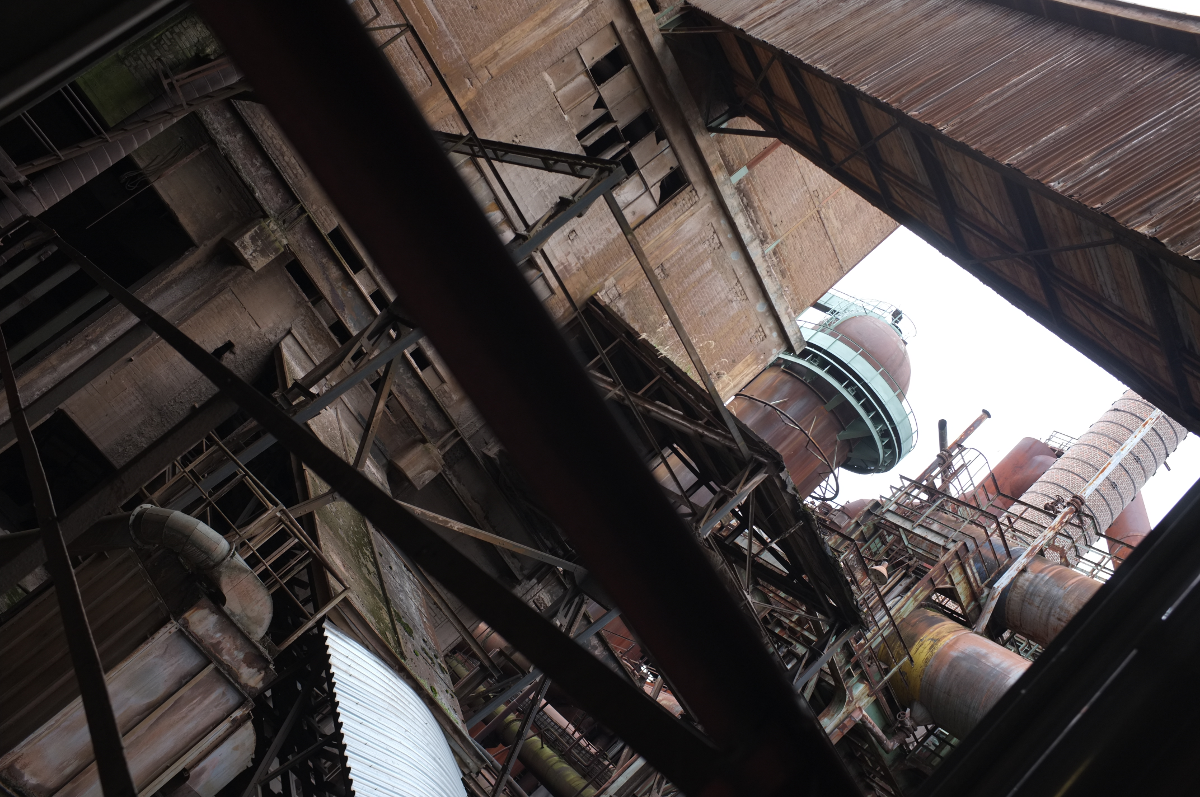
\includegraphics[width=0.7\textwidth]{Examples/example_5.png}
  \caption{Erstes Bild, Völklinger Hütte}
  \label{fig:Huette}
\end{figure}


\subsection{Wrapfigure}
Abbildung~\ref{fig:Huette} ist zwar ganz nett anzusehen, aber vielleicht sähe es eleganter aus, wenn die Abbildung 
von unserem Textabschnitt umflossen werden würde. Diese Art von Abbildungen sollte jedoch sparsam und mit großer Sorgfalt eingesetzt werden, da es zu unschönen Darstellungen kommen kann.
\blindtext
\begin{wrapfigure}{l}{0.4\textwidth}
  \centering
  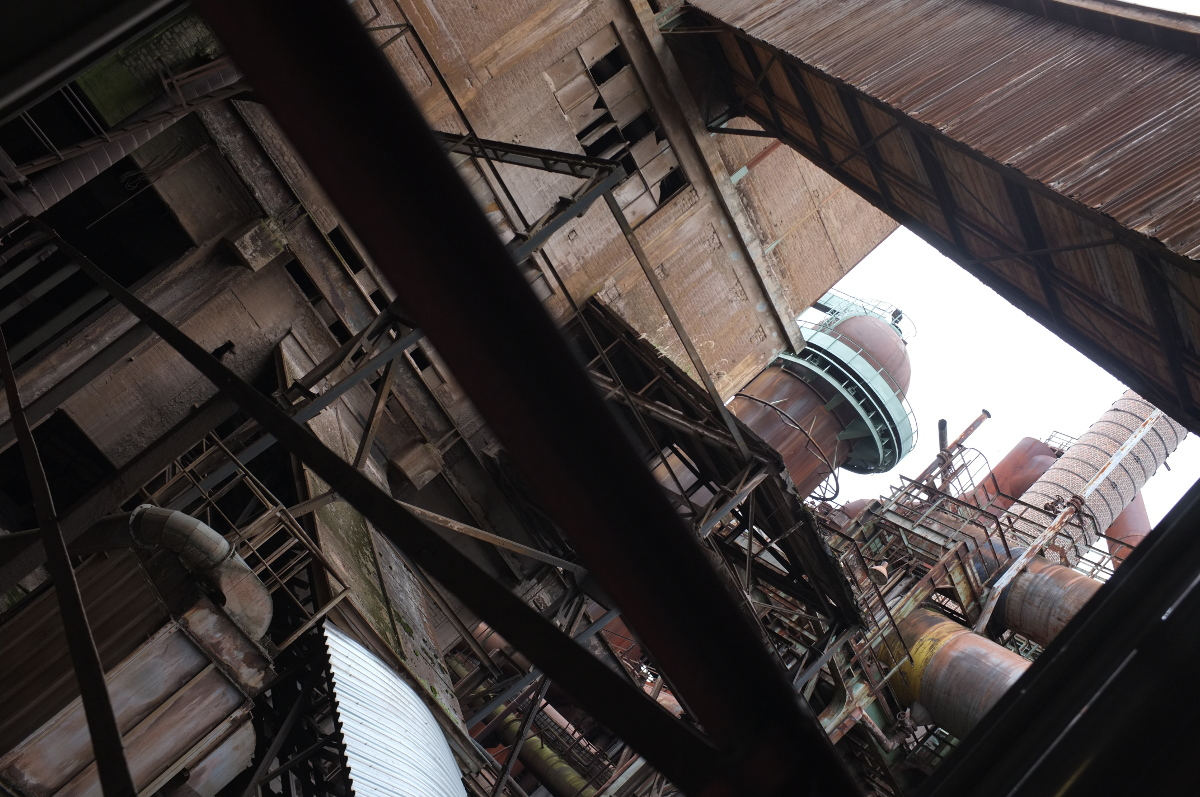
\includegraphics[width=0.4\textwidth]{Examples/example_5.jpg}
  \caption{Völklinger Hütte, *.jpg}
  \label{fig:Huette2}
\end{wrapfigure}
\blindtext


\subsection{Subfigures}
Es ist ebenso möglich, mehrere Abbildungen nebeneinander zu setzen, wie in Abbildung~\ref{fig:Beide} zu sehen ist. Eine separate Referenzierung ist auch möglich: Abbildung~\ref{subfig:abbone}.
\begin{figure}[bth]
  \subfloat[Erstes ...]{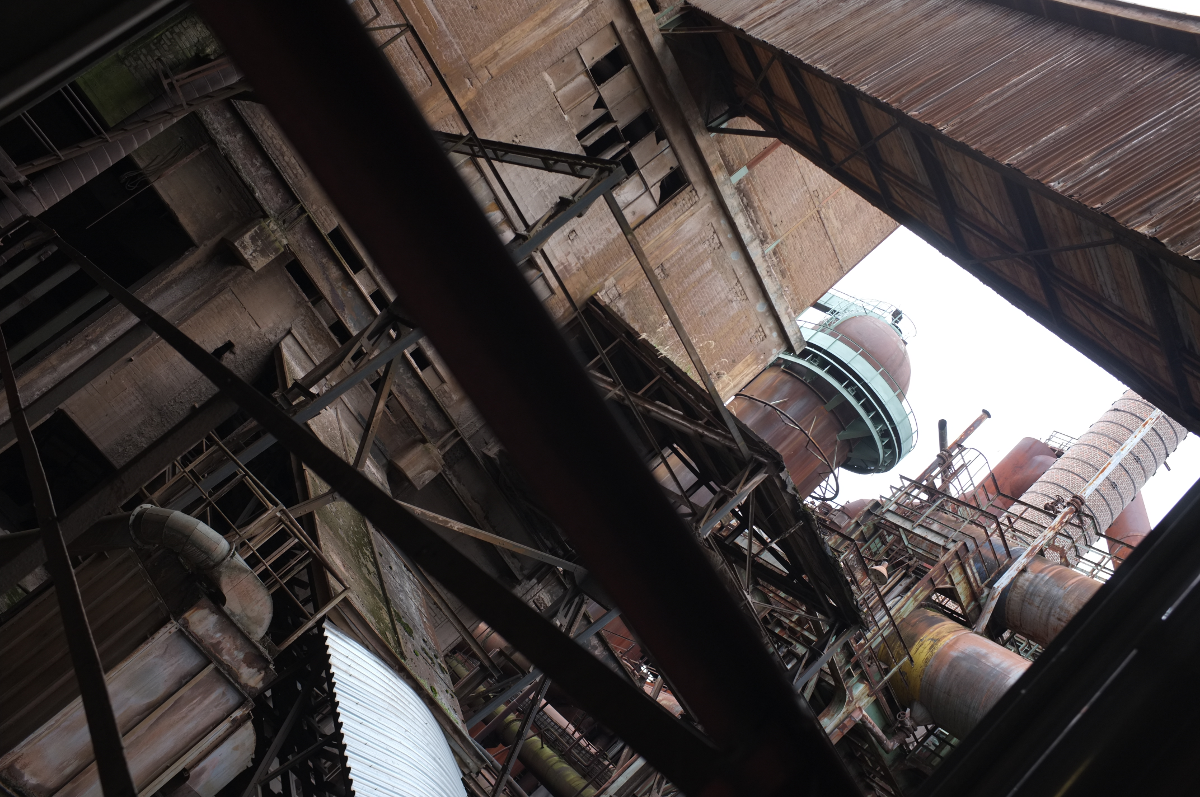
\includegraphics[width=0.49\textwidth]{Examples/example_5.png}\label{subfig:abbone}}\hfill
  \subfloat[... und zweites Bild]{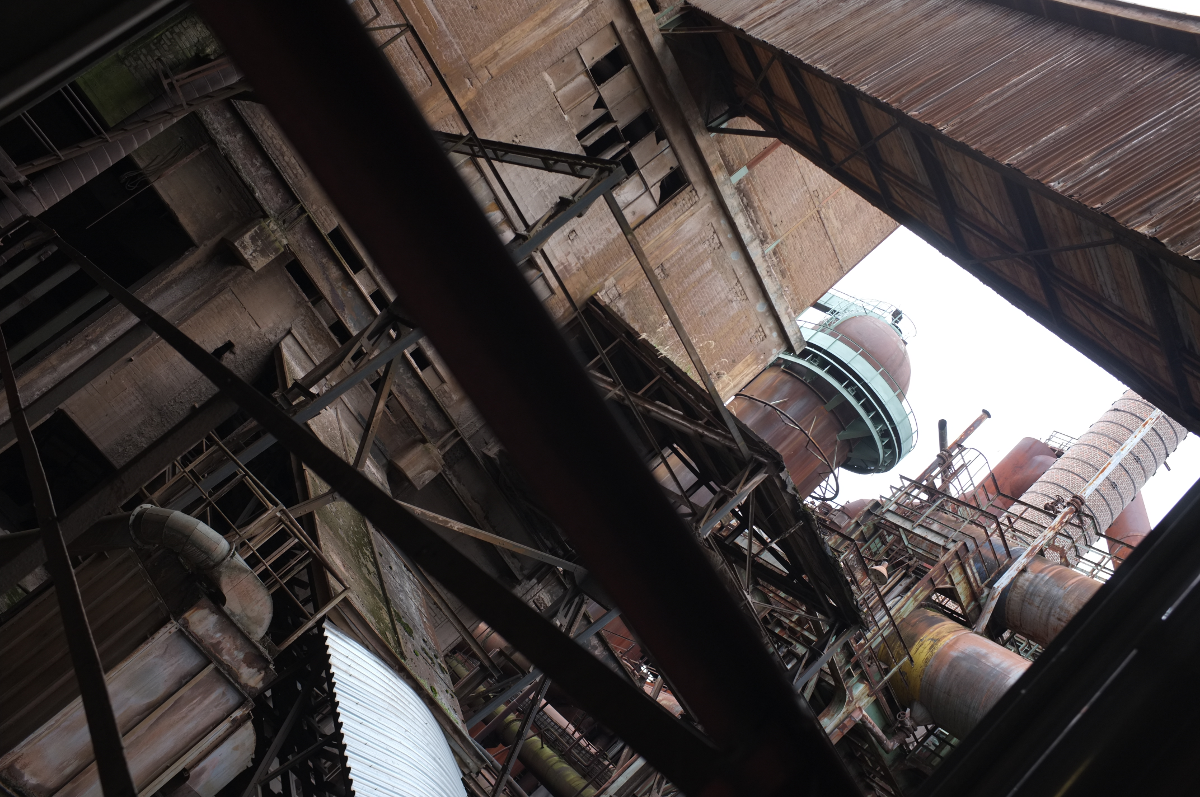
\includegraphics[width=0.49\textwidth]{Examples/example_5.png}\label{subfig:abbtwo}}
  \caption{Mehrere Abbildungen nebeneinander}
  \label{fig:Beide}
\end{figure}


\subsection{Qualitätsunterschiede}
\begin{figure}[p]
	\centering
  \subfloat[\textit{PDF}-Format]{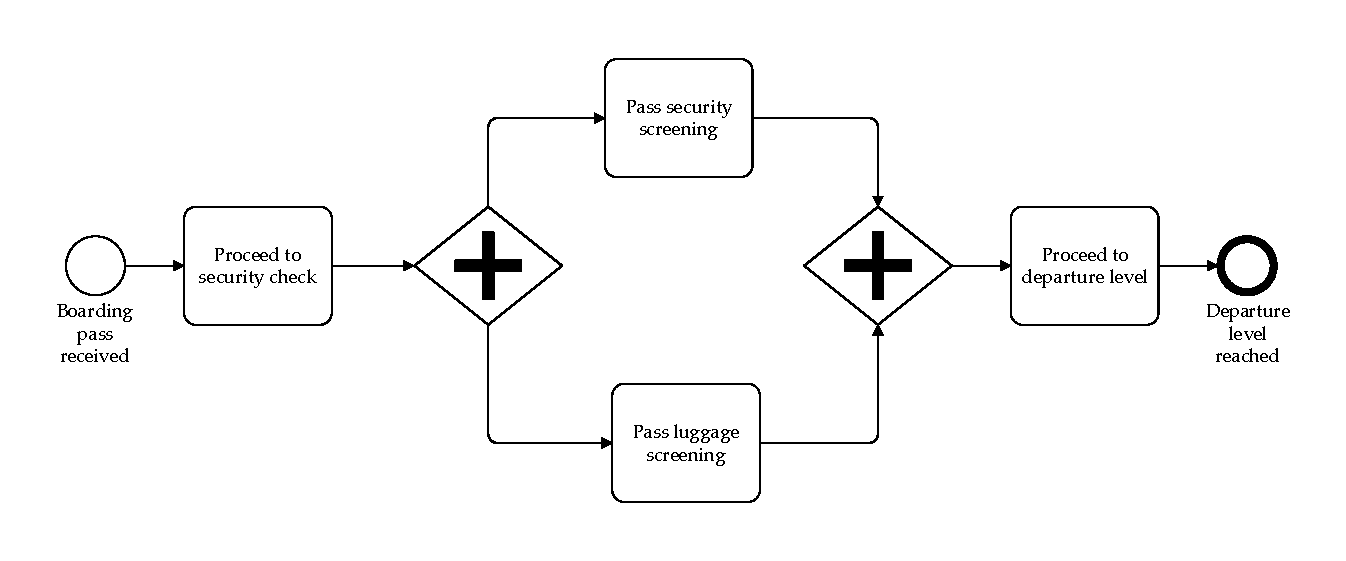
\includegraphics[width=0.65\textwidth]{Examples/bpmn.pdf}} \\
  \subfloat[\textit{JPG}-Format]{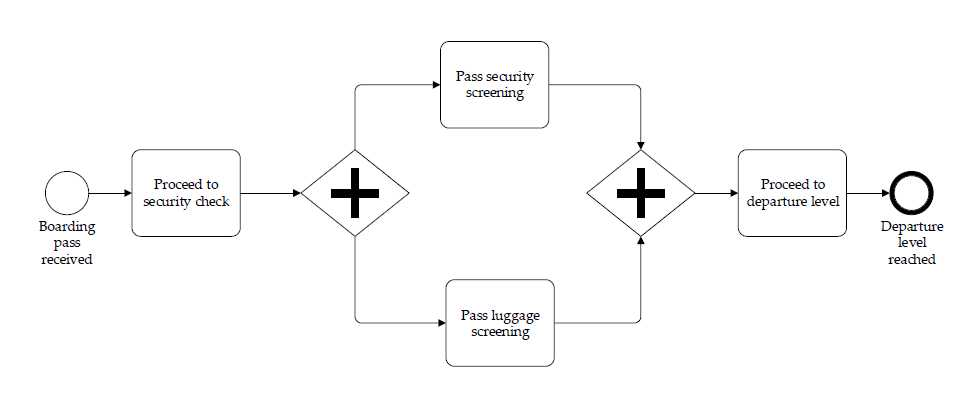
\includegraphics[width=0.65\textwidth]{Examples/bpmn.jpg}}
  \caption{Beide Formate im Vergleich}
  \label{fig:pdfvsjpg}
\end{figure}

\begin{figure}[p]
	\centering
  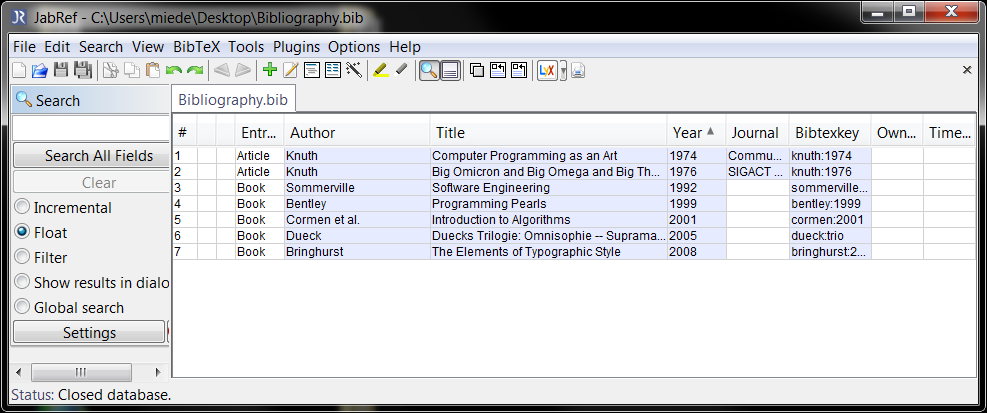
\includegraphics[width=0.65\textwidth]{Examples/jabref.png}
   \caption{\textit{PNG}-Format}
  \label{fig:pngvsjpg1}
\end{figure}

\begin{figure}[p]
	\centering
  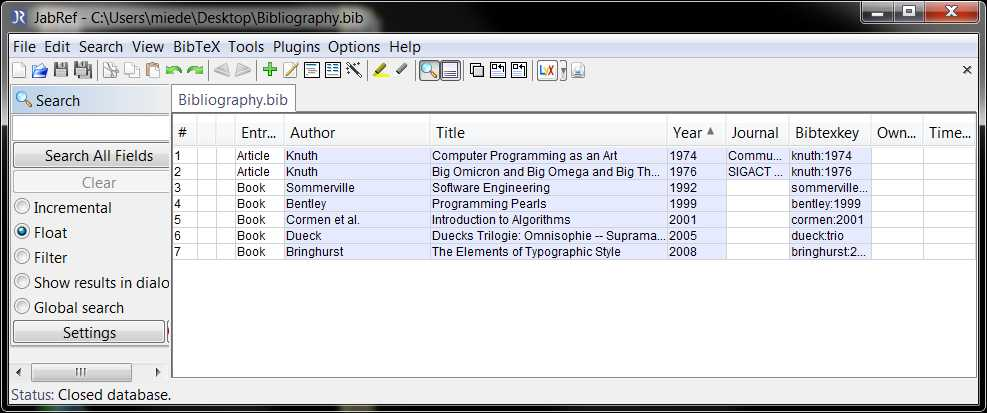
\includegraphics[width=0.65\textwidth]{Examples/jabref.jpg}
   \caption{\textit{JPG}-Format}
  \label{fig:pngvsjpg2}
\end{figure}

Leider haben die unterschiedlichen Grafikformate bedingt durch die unterschiedlichen Kompressionsverfahren einige Schwächen, insbesondere die Umwandlung in das \textit{JPG}-Format erzeugt unangenehme Artefakte im Bild. \autoref{fig:pdfvsjpg} zeigt die Unterschiede zwischen \textit{PDF-Format} und \textit{JPG-Format} im Vergleich. 

Wenn eine \textit{*.pdf}-Datei nicht infrage kommt, beispielsweise bei Screenshots, ist unbedingt das \textit{PNG-Format} vorzuziehen. 
Den Unterschied machen \autoref{fig:pngvsjpg1} und \autoref{fig:pngvsjpg2} deutlich.

\glqq Faustregeln\grqq im Umgang mit Abbildungen:
\begin{itemize}
	\item Diagramme bzw. alles, was Linien usw. enthält: \textit{PDF} (im Vektorformat).
	\item Screenshots bzw. alles, was größere gleichfarbige Flächen enthält: \textit{PNG}.
	\item Der Rest (in der Regel Fotos): \textit{JPEG}.
\end{itemize}





%*******************************
% 			Listings 		   *
%*******************************

\section{Quellcode einbinden}
Das Package \textit{lstlisting} ermöglicht es, Quellcode ansprechend in das Dokument einzubinden. Man kann Quellcode einzeilig einbinden 
mittels \lstinline{\lstinline|Quellcode|}. Dabei ist darauf zu achten, dass der Befehl einmal mit \{ \} und einmal mit | | aufgerufen werden kann, je nachdem, 
welche Zeichen im angegebenen Quelltext genutzt werden. 
Es ist auch möglich eine eigene Umgebung für Quelltext zu schaffen:

\begin{lstlisting}[caption=Erstes Listing,style=Java]
private Umgebung(int i, int k)
{
	System.out.println("Eine Funktion mit " + i + "und" + k ".");
}
\end{lstlisting}  

Wer Quelltext aus externen Dateien einbinden möchte, geht wie folgt vor:

\lstinputlisting
[caption={Externer Quellcode},style=Java]
{Examples/Code.java}

Wie genau der Quellcode formatiert und gefärbt ist, ist in \textit{htwsaar.i.mst.config.tex} hinterlegt, wobei fü verschiedene Sprachen auch eigene Styles angelegt werden
können (hier z.B. für Java).
\section{Mathematische Ausdrücke}
Mathematische Ausdrücke sind eine kleine Kunst für sich. Am allereinfachsten kann man eine Formel, wie \(a + b = c\) in den Fließtext einbinden, wobei LaTeX die Höhe der Ausdrücke der Zeile anpasst,
wie hier zu sehen \(\sum_{y=0}^{x} a\) . In einer Umgebung sieht das schon anders aus:
\begin{equation}
  \sum_{y=0}^{x} a
\end{equation}

Griechische Buchstaben:
\begin{equation}
	\alpha\beta\gamma\delta\epsilon\varepsilon\zeta\eta
	\theta\iota\kappa\lambda\mu\nu\xi\pi\varpi\rho\varrho
	\sigma\tau\upsilon\phi\varphi\chi\psi\omega
\end{equation}

Brüche:
\begin{equation}
	Ergebnis = \frac{a}{b}
\end{equation}

\begin{equation}
	\frac{\sin{\alpha}^2 + \cos{\alpha}^2}{1} = 1
\end{equation}

\begin{equation}
	\frac{-9x}{\frac{2y}{3z+2}}
\end{equation}

Text innerhalb von Formeln:
\begin{equation}
\sum_{y=1}^{n} y = \frac{n*(n+1)}{2}
\quad
\text{Gaußsche Summenformel}
\end{equation}

Hoch- bzw. Tiefstellungen:
\begin{equation}
	x_{i,j}^2
\end{equation}

\begin{equation}
	{x_{i,j}}^2
\end{equation}

\begin{equation}
	x_{n_0}
\end{equation}


Matrizen:
Matrizen werden innerhalb der mathematischen Umgebung als wiederum neue Umgebung eingebunden. Wie bei Tabellen auch werden Zeilen durch \lstinline{\\} und Spalten durch \lstinline{&} getrennt.

\begin{equation}
	\begin{pmatrix} 
		a&b\\
		c&d 
	\end{pmatrix}
\end{equation} 

\begin{equation}
	\begin{vmatrix} 
		a&b\\
		c&d 
	\end{vmatrix}
\end{equation} 

Fallunterscheidung:
\begin{equation}
	f(x) = 
	\begin{cases}
		0, &\text{falls } x < 0 \\
		1, &\text{falls } x \geq 0
	\end{cases}
\end{equation}




%############################################################
\clearpage\section{To-Do-Notes}
Um bei einer längeren Arbeit nicht den Überblick zu verlieren, an welcher Stelle es nötig ist
weiter zu arbeiten, bietet es sich an, kleine Notizen einzufügen. Das Package \textit{todonotes}
stellt eine elegante Lösung bereit, um differenziert und vielfarbig jene Abschnitte zu kennzeichnen,
die einer weiteren Bearbeitung bedürfen.

\subsection*{Beispiel für To-Do-Notes}
Dies hier ist ein Blindtext zum Testen von Textausgaben. Wer diesen Text liest, ist selbst
\todo{Wie weit geht diese Bezeichnung?} schuld. Der Text gibt lediglich den Grauwert der Schrift an. Ist das wirklich so? Ist es
gleichgültig, ob ich schreibe: Dies ist ein Blindtext? oder Huardest gefburn? Kjift?
mitnichten! Ein Blindtext bietet mir wichtige Informationen. An ihm messe ich die Les-
barkeit einer Schrift, ihre Anmutung, \todo{Plain todonotes.}wie harmonisch die Figuren zueinander stehen
und prüfe, wie breit oder schmal sie läuft. Ein Blindtext sollte möglichst viele verschie-
dene Buchstaben enthalten und in der Originalsprache gesetzt sein. Er muss keinen
Sinn ergeben, sollte aber lesbar sein.\todo[nolist]{Todonote that is only shown in the margin and not in
the list of todos.}%
Fremdsprachige Texte wie Lorem ipsum dienen
nicht dem eigentlichen Zweck, da sie eine falsche Anmutung vermitteln. Dies hier ist
ein Blindtext zum Testen von Textausgaben. Wer diesen Text liest, ist selbst schuld. 

\todo[inline]{A very long todonote that certainly will fill more
than a single line in the list of todos. Just to make sure let's add
some more text \ldots}

Der Text gibt lediglich den Grauwert der Schrift an. Ist das wirklich so? Ist es gleichgültig,
ob ich schreibe: Dies ist ein Blindtext? oder Huardest gefburn? Kjift? mitnichten!
\todo[noline]{A note with no line back to the text.}
Ein Blindtext bietet mir wichtige Informationen. An ihm messe ich die Lesbarkeit einer
Schrift, ihre Anmutung, wie harmonisch die Figuren zueinander stehen und prüfe, wie
\todo[caption={A short entry in the list of todos}]{A very long
todonote that certainly will fill more than a single line in the
list of todos \ldots}
breit oder schmal sie läuft. Ein Blindtext sollte möglichst viele verschiedene Buchstaben
enthalten und in der Originalsprache gesetzt sein. Er muss keinen Sinn ergeben, sollte
aber lesbar sein. Fremdsprachige Texte wie Lorem ipsum dienen nicht dem eigentlichen Zweck, 
da sie eine falsche Anmutung vermitteln.
\missingfigure{A figure I have to make \ldots}

%Nummerierte ToDo-Notes
\todox{Erste Nummer...}
\todox{Zweite Nummer...}

%Alles To-Dos als Liste ausgegeben
Nachfolgend wird noch eine Liste aller To-Dos auf einer separaten 
Seite ausgegeben.
%\begingroup
	%\let\clearpage\relax
	%\let\cleardoublepage\relax
    	\listoftodos
%\endgroup 


 		% Abschlussarbeit geht!


%<<< Hier alle Chapter der Abschlussarbeit (einzeln) einbinden

%Einleitung
\cleardoublepage%=========================================
% 	   Einleitung     		 =
%=========================================
\chapter{Einleitung}

\section{Motivation}
Im Informationszeitalter werden Informationen meist über alles andere gestellt. Wir bleiben allerdings physisch und unsere Umgebung ebenso. Um Computer in diesen physischen Umgebungen zu nutzen, sind viel zu oft noch Informationen von Menschen nötig. Menschen haben allerdings eine limitierte Aufmerksamkeitsspanne, Zeit und Genauigkeit. Computer sind von Informationen abhängig, die von Menschen erstellt, aufgenommen oder eingetippt werden. Menschen brauchen Zeit um Werte aufzunehmen und machen Fehler dabei. Dies führt dazu, dass Computer ebenso fehlerhafte Daten produzieren oder Informationen erst zu spät zur Verfügung stehen. Oft führt 
Computer und Sensoren haben keine schwankende Aufmerksamkeitsspanne und werden nicht müde. Eine Lösung wäre folglich eine Kommunikation zwischen der physischen Welt und der digitalen Welt, ohne den Mensch als Informations Brücke. Dies ist das Ziel der \textit{Internet of Things}. Eine einheitliche Definition des Begriffs Internet of Things existiert nicht. Denn es gibt unterschiedliche Auffassungen davon, was zu den Internet of Things gezählt wird. Maschinelle Sensoren im Bereich der Industrie 4.0 gelten als selbstverständlich, aber man könnte auch sogenannte RFID Tags oder sogar Smartphones hinzuzählen. Ich werde mich hier auf die Definition von Forrest Stroud beziehen: 
\begin{quote}
„The IoT refers to the ever-growing network of physical objects that feature an IP address for the internet connectivity and the communication that occurs between these objects and other internet-enabled devices and systems.“ 
\end{quote}
Stroud bezieht sich demnach auf physische Objekte, welche eine IP-Adresse zur Kommunikation vorweisen. Diese reichen von Geräten der Infrastruktur, wie Ampelanlagen und 

\section{Aufgabenstellung und Zielsetzung}
In meiner Arbeit werde ich Xamarin, React Native, Ionic und Flutter miteinander vergleichen und eine passende Lösung für die Problemstellung des IoT-Testfelds der HTWSaar auswählen. Anschließend wird mit dieser ein Frontend für das SmartCity-Testfeld konzipiert und umgesetzt. Dabei ist das Ziel eine Struktur zu entwickeln, mit welcher eine einfache Erweiterbarkeit und Modifikation erreicht wird. Konkret soll es möglich sein, weitere Use Cases einzubinden. Dadurch wird die Applikation zukunftssicher und flexibel. Zudem kann das SmartCity Testfeld erweitert werden, ohne das ein weiteres Frontend entworfen werden muss. Die erarbeiteten Konzepte sollen anhand einer Proof of Concept Implementierung getestet werden. Dabei wird zunächst eine Frontend-Implementierung des Projekts \textit{Smart-Garbage} erarbeitet.

\section{Struktur der Arbeit}
Diese Arbeit ist wie Folgt strukturiert. Zunächst wird in Kapitel eine Basis an Grundwissen gesammelt. Hierzu zählen eine Betrachtung der verschiedenen 




%Grundlagen
\cleardoublepage%=========================================
% 	   Grundlagen     		 =
%=========================================
\chapter{Grundlagen}
\label{ch:grundlagen}
Um die Cloud-Native-Architektur zu betrachten, gilt es erst einige Grundlagen zu erarbeiten. In diesem Kapitel wird zunächst der Begriff Cloud abgegrenzt. Dabei wird auch der Unterschied von \textit{Public} und \textit{Private Cloud} betrachtet. Daraus wird anschließend eine Liste von Anforderungen an eine Cloud-Architektur formuliert. Aufbauend auf dieser wird abschließend die Cloud Native Architektur definiert und deren Eigenschaften betrachtet. 

\section{Die Cloud}
Der Begriff Cloud ist heutzutage sowohl in Fachliteratur, als auch in IT-fernen Bereichen vorzufinden. Dabei wird der Begriff \textit{Cloud} als Oberbegriff für neue Technologien und Produkte verwendet.\\ 
Dafür gilt es zunächst zu ermitteln, in welcher Umgebung Cloud-Applikationen betrieben werden.\\\\
Das National Institute of Standards and Technology (NIST) definiert \textit{Cloud Computing}, als ein Model für allgegenwärtigen Zugriff auf eine geteilte Menge von Rechenleistung . Der all-gegenwärtige Zugriff wird durch einen sogenannten \textit{Service-Provider} bereitgestellt. Der Kunde kann demnach flexibel Rechenleistung dazu kaufen, oder die bereitgestellte Rechenleistung verringern. Hierfür ist keine menschliche Kommunikation von Nöten. Deshalb wird dies von der NIST als \textit{On-demand self-service} bezeichnet.\\
Um On-demand self-service zu ermöglichen, nutzt der Service-Provider das sogenannte \textit{Resource-Pooling}. Hierfür teilt der Service-Provider dem Kunden automatisiert Rechenleistung zu. Der Kunde hat hierbei nur begrenzt Einfluss auf den Standort oder die genaue Maschine, welche die Leistung zur Verfügung stellt.\cite{mell_nist_2011}\\
Der Kunde bezahlt folglich für Rechenleistung, und nicht für einzelne Maschinen. Die Cloud kann demnach als Paradigma für das Bereitstellen von Services über das Internet gesehen werden \cite{avram_advantages_2014}.

\subsection{Service Modelle}
Verschiedene Geschäftsmodelle des Cloud-Computings setzen unterschiedliche Grade der Abstraktion um. Hierbei wird zwischen den Service Modellen \textit{Infrastructure as a Service}, \textit{Plattform as a Service} und \textit{Software as a Service} unterschieden. Im Nachfolgenden werden diese Modelle voneinander abgegrenzt.
\subsubsection{Infrastructure as a Service}
Das sogenannte\textit{ Infrastructure as a Service (IaaS)}\cite{mell_nist_2011} stellt Speicher -und Rechenleistung zur Verfügung. Der Kunde muss also nicht selbst physische Hardware betreiben. IaaS kann als Grundschicht unter allen anderen Service Modellen gesehen werden.\\
Mittels Virtualisierung teilt der Service-Provider die physische Hardware auf und teilt sie den Kunden zu. Der  Kunde hat also kein Einfluss auf die zugrundeliegende Infrastruktur. Allerdings kann er Aspekte wie Speicher, Betriebssystem, Middle-Ware und die Anwendung selbst konfigurieren \cite{dimpi_rani_rajiv_kumar_ranjan_comparative_2014}.\\
Auch ein begrenzter Zugriff auf Netzwerkomponenten, wie zum Beispiel die Firewall, kann möglich sein. IaaS stellt demnach die selben Funktionen wie ein traditionelles  Rechen-Center zur Verfügung. Der Kunde muss allerdings kein solches Instandhalten und kann flexibel die Rechenleistung erhöhen oder verringern. \\
Abgerechnet wird in der Regel entsprechend der Nutzungsdauer. In einigen Fällen übernimmt der Service-Provider auch Aufgaben wie die Systemwartung, Datensicherung und das Notfall-Management.\\
Unter anderem sind Microsoft, IBM und Amazon Anbieter von IaaS Angeboten. \cite{simon_lohmann_iaas_nodate} \cite{mell_nist_2011}
\subsubsection{Plattform as a Service}
Das \textit{Plattform as a Service (PaaS)}\cite{mell_nist_2011} Model abstrahiert gegenüber IaaS weitere Aspekte der Cloud. Weiterhin muss der Kunde keine eigene Rechenzentren verwalten und erhält durch den Service Provider flexibel Rechenleistung.\\
Allerdings werden nun auch Aspekte wie das Betriebssystem, die Speicherverwaltung mit Datenbanken und das Netzwerk, durch den Service Provider verwaltet. Der Kunde erhält eine Entwicklungsumgebung in der Cloud, über welche der die Anwendung bereitstellen kann. \\
PaaS ist dafür konzipiert den kompletten Lebenszyklus einer Anwendung zu ermöglichen. Hierzu zählen das bauen, testen, veröffentlichen, verwalten und aktualisieren einer Anwendung \cite{dimpi_rani_rajiv_kumar_ranjan_comparative_2014}. Auf einer höheren Abstraktion kommen neben Entwicklungswerkzeugen, Programmiersprachen, Bibliotheken und Datenbanken auch Container-Techniken dazu.\\
Zu den wichtigsten PaaS Anbietern gehören Amazon, IBM und Microsoft. \cite{simon_lohmann_platform_nodate}\cite{sowmya_layers_2014} \cite{mell_nist_2011} 
\subsubsection{Software as a Service}
\textit{Software as a Service (SaaS)} ist die am meisten abstrahierte Form des Cloud-Computings. Kunden können über das Internet auf Angebote zugreifen, welche von einem Service-Provider zur Verfügung gestellt werden. Die Applikation wird durch den Service-Provider verwaltet, betrieben und aktualisiert. \\
Der Nutzer verwaltet keinen Aspekte der zugrundeliegenden Infrastruktur. Einzig eine konfigurieren der Anwendung selbst kann möglich sein.\\
Typische SaaS-Applikationen im Business Bereich sind \textit{Google G Suite} \cite{noauthor_google_nodate}  und \textit{Microsoft Office 365} \cite{noauthor_office_nodate}. \\
SaaS-Provider rechnen Anwendungen in der Regen anhand bestimmter Parameter, wie die Anzahl der Nutzer, ab. Auch bei SaaS-Angeboten können Kunden bei Bedarf einzelne Dienste oder Funktionen stärker in Anspruch nehmen. \cite{wolfgang_herrmann_saas_nodate} \cite{sowmya_layers_2014} \cite{mell_nist_2011}

\subsection{Deployment Modelle}
Neben dem Grad der Abstraktion stellt auch der Ort der Hardware eine Rolle. Wird diese lokal von dem eigenen Unternehmen verwaltet? Oder ist eine externe Firma dafür verantwortlich? Hierfür existieren einige Modell, welche im Folgenden voneinander differenziert werden:
\begin{description}
    \item [on premise] \hfill \\ Auch als on-premise Cloud oder private Cloud bezeichnet \cite{dimpi_rani_rajiv_kumar_ranjan_comparative_2014}. Die Infrastruktur wird exklusiv von einer Organisation genutzt \cite{mell_nist_2011}. Die Verwaltung der Infrastruktur kann ebenfalls durch diese Organisation erfolgen. Alternativ kann eine externe Firma damit beauftragt werden. Die benötigte Hardware befindet sich entweder in-house (\textit{on-premise}) oder oder wird \textit{off-premise} extern bereitgestellt \cite{zwicker_saas_nodate}.
    \item [public Cloud] \hfill \\ Die Infrastruktur wird durch einen Dritt-Anbieter über das Internet zur Verfügung gestellt. Die gesamte Hardware ist im Besitzt des Service-Providers. Die selbe Hardware, Speicher und Netzwerk-Geräte des Service-Providers werden mit anderen Kunden geteilt. Beispiele hierfür wären Microsoft Azure oder Amazon Web Services. \cite{microsoft_public_nodate} \cite{mell_nist_2011}
    \item [hybrid Cloud] \hfill \\ Hybrid Clouds bestehen aus mehreren getrennten Cloud-Infrastrukturen. Daten und Applikationen einer hybrid Cloud können zwischen private Cloud und public Cloud Infrastrukturen wechseln. \cite{mell_nist_2011}
\end{description}

\subsection{Vorteile und Möglichkeiten der Cloud}
Jedes der oben genannten Deployment Modelle und Service Modelle hat eine Menge von Eigenschaften gemeinsam. Avram et al. nennt folgende Eigenschaften: (i) pay-per-use (kein fortlaufenden Verpflichtungen), (ii) elastic capacity and the illusion of infinite resources; (iii) self-service-interface; und (iv) resources that are abstracted or virtualized \cite{avram_advantages_2014}. Aus diesen folgend direkt einige Vorteile des Cloud-Computings.
\begin{itemize}
  \item Durch das pay-per-use Modell muss der Kunde nur für die Leistung zahlen, die er tatsächlich benötigt. Dies reduziert Hardware-Kosten, wie auch die Kosten für Verwaltung, Software-Updates und den Strom. Ferner wird weniger Personal für die Verwaltung der IT benötigt. Dies ermöglicht auch kleineren Firmen rechen-aufwändige Analysen zu bewältigen. Letztere waren zuvor nur größeren Firmen vorbehalten. Diese umfangreichen Berechnungen benötigen meist viel Leistung, für einen kurzen Zeitraum. Durch das self-service-interface (iii) und die dynamische Kapazität von Leistung (iv) mit pay-per-use (i) ist dies möglich. Avram et al \cite{avram_advantages_2014} sieht hier zusätzlich eine Möglichkeit für Dritte-Welt-Länder zu dem Westen aufzuschließen. Länder welche traditionell nicht die benötigen Ressourcen gehabt hätten, können nun diese durch Cloud-Computing beziehen.  
  \item Durch das Cloud-Computing können neue Business-Modell umgesetzt werden. Die Cloud ermöglicht einen direkten Zugriff auf Rechenleistung, ohne eine Vorherige Kapital-Anlage des Kunden \cite{noauthor_premise_2020}. Es muss nicht zuvor Geld in ein Rechenzentrum oder zusätzliche IT-Experten investiert werden. Die Zeit bis ein neues Produkt gewinnbringend an den Markt gebracht werden kann, ist demnach deutlich gesunken. Viele Internet-Startups konnten dadurch gegründet und zum Erfolg geführt werden \cite{avram_advantages_2014}. 
  \item Cloud-Computing erleichtert es Firmen, ihre Services zu skalieren. Wächst die Zahl der Nutzer, kann Rechenleistung dazu gekauft werden. Die Kosten steigen daher dynamisch mit der Reichweite des Unternehmens. Auch eine Reaktion auf ein kurzfristigen Anstieg oder Abfall der Nutzer-Anfragen ist möglich. Eines der Ziele des Cloud-Computings besteht darin, Ressourcen mithilfe von Software-APIs je nach Client-Auslastung bei minimaler Interaktion mit dem Service-Provider dynamisch zu vergrößern oder zu verkleinern \cite{avram_advantages_2014}. Dies ist möglich, da die Rechen-Ressourcen durch Software verwaltet werden. Für eine dynamische Skalierung, wird zusätzlich eine passende Software-Architektur benötigt. Hierauf wird in einem späteren Kapitel eingegangen.
  \item Hier ist außerdem der Gedanke aufzugreifen, dass eine Fokussierung auf das Geschäftsmodell möglich wird. Firmen können sich auf ihr eigentliches Geschäftsmodell konzentrieren. Zeit und Geld können in das Geschäftsmodell und nicht in die IT-Infrastruktur investiert werden.
\end{itemize}

\section{Anforderungen}
Nachdem wir im letzten Abschnitt den Begriff Cloud-Computing erläutert haben, gilt es nun Cloud-Applikationen zu betrachten. Die meisten der zuvor genannten Vorteile des Cloud-Computings können nur durch eine passende Software-Architektur vollkommen ausgeschöpft werden. Beim Entwurf der Architektur einer Cloud-Applikation müssen einige Aspekte beachtet werden. Folgende Anforderungen haben sich dabei herauskristallisiert:
\begin{itemize}
    \item Cloud-Applikationen operieren meist global. Dies heißt nicht nur, dass der Dienst stets über das Internet erreichbar ist. Bei der Betrachtung von globalem Zugriff muss berücksichtigt werden, dass der Dienst in lokalen Rechenzentren dupliziert werden muss \cite{gannon_cloud-native_2017}. Nur so kann eine geringe Latenz garantiert werden. Dabei führt die Integrität von Daten häufig zu Problem. Die persönlichen Daten müssen dem Nutzer stets zur Verfügung stehen. Dem Nutzer darf nicht ersichtlich sein, dass seine Daten an mehreren Orten abgespeichert sind.  
    \item Cloud-Applikationen müssen mit vielen tausend von parallelen Nutzern operieren können. Neben einer vertikalen Skalierung (mehr und bessere Hardware) wird demnach auch eine horizontale Skalierung nötig \cite{gannon_cloud-native_2017}. Diese wird meist durch Parallelisierung umgesetzt. Eine horizontale Skalierung führt erneut zu einem Fokus auf die Konsistenz und Synchronisation des Systems. 
    \item Die Architektur einer Cloud-Applikationen muss mit der Annahme entwickelt werden, dass die Hardware nicht konstant ist und Fehler vorkommen werden \cite{gannon_cloud-native_2017}. Gannon et Al. \cite{gannon_cloud-native_2017} sieht Probleme bei Applikationen, welche nicht für die Cloud entwickelt wurden. Diese nehmen an, dass die Hardware und das Betriebssystem konstant sind. Der kleinste Fehler im Rechenzentrum oder des Netzwerks führt hier bereits zu Fehlern. 
    \item Cloud-Applikationen müssen die Anforderungen an Verteilte-Systeme beachten \cite{scholl_cloud_2019}. Als Beispiel soll das sogenannte CAP-Theorem erwähnt werden \cite{julianbrowne_brewers_nodate}. Ohne eine Optimierung für den Ausfall einzelner (Teil-)Systeme ist die Anforderung \textit{Partition Tolerance} des CAP-Theorem nicht erfüllt. Es stellt sich also heraus, dass verteilte Systeme eine Reihe von Anforderungen mit sich bringen. Die Architektur muss demnach damit umgehen, dass sich Dienste nicht auf der selben Maschine befinden. Es wird folglich mit einem Netzwerk von Maschinen gearbeitet. Es wird die Welt der Verteilten Systeme betreten. Diese bringt eine Reihe von eigenen Anforderungen mit sich. Oft werden hier Falsch-Annahmen gemacht. Scholl et Al. \cite{scholl_cloud_2019} nennt diese Annahmen  \textit{Fallacies of Distributed Systems}. Dazu gehören Aussagen wie unter Anderem ``the Network is reliable'', ``Latency is zero'' oder ``There is infinite bandwith''. All diese Aspekte führen zu eigenen Anforderungen, welche die Architektur beachten muss.
    \item Die meisten Cloud-Applikationen werden für den Dauerbetrieb entwickelt. Ein zugriff der Nutzer soll stets möglich sein. Hier ist außerdem der Gedanke aufzugreifen, dass Firmen  Verträge mit dem Kunden haben können. Diese beschränken eine mögliche Ausfallzeit auf wenige Stunden im Jahr. Ein Einspielen von Updates darf demzufolge nicht zu einer Downtime für den Nutzer führen. Zudem müssen diese Updates stets getestet werden. Auch Fehler im System oder Abstürze einzelner Knoten dürfen nicht das gesamte System, oder einzelne Funktionen dessen, lahmlegen. Ein umfangreiche Überwachung des Systems und das vorhalten von Ersatzkonten sind nur einige der wichtigen Operationen.\cite{gannon_cloud-native_2017}
\end{itemize}
Zusammenfassend lässt sich sagen, dass Entwickler und Software-Architekten drei großen Herausforderungen der Cloud gegenüber stehen. Zunächst müssen sie verteilte Systeme verstehen. Eine Anforderungen, welche so vorher schon relevant war, allerdings nun noch prominenter in den Vordergrund dritt. Ferner müssen sich Entwickler mit neuen Technologien wie Containern vertraut machen. Und abschließend müssen sie sich bewusst werden, welche Entwurfsmuster in der Cloud funktionieren.

\section{Prinzipien einer Cloud Native Architektur}
Nachdem nun die Begriffe Cloud-Computing und Cloud-Applikationen beleuchtet wurde, kann eine Architektur für die Cloud betrachtet werden. Das Ziel dieser ist, die Möglichkeiten der Cloud maximal zu Nutzen. Traditionelle Infrastrukturen (on-premise Service Modelle) fokussieren sich auf eine feste Anzahl an Hardware-Komponenten und deren Leistung. Der Cloud-Service-Provider teilt die Leistung allerdings flexibel zu. Folglich nutzen Cloud-Native Architekturen Prinzipien, wie das horizontale Skalieren und automatische Ersetzen von abgestürzten Komponenten um Leistung und Elastizität bereit zu stellen.\\
Sowohl Scholl et Al.\cite{scholl_cloud_2019} , als auch Microsoft, Amazon und Google \cite{tom_grey_5_nodate} definieren eine Vielzahl von Eigenschaften einer Cloud-Native Architektur. Im Folgenden werden diese Eigenschaften beleuchtet. 
\subsection{Automatisierung}
Eines der Ziele einer Cloud-Native Architektur ist es, so viele Aspekte des Systems wie möglich zu automatisieren. Scholl et Al.\cite{scholl_cloud_2019} bezeichnet diese Eigenschaft als ''Operational Excellence''. Ganz natürlich kommt hier das Continuous Integration / Continuous Delivery (CI/CD) ins Spiel. CI/CD beschreibt das automatisierte bauen, testen und deployen des Systems. Auch das Zurücksetzen von Updates (\textit{Rollback}) sollte automatisiert werden.\\
Neben diesen Apsekten ist auch das Logging zentral. \\
Eine Überwachung der Anwendung sollte ebenfalls Implementiert werden. Diese führt dazu, dass Fehler frühzeitig erkannt werden können. Darüber hinaus hat diese auch weitere Vorteile.\\
Aspekte der Cloud wie das on-demmand-self-service ermöglichen es, im Code der Anwendung selbst, die Umgebung der Anwendung anzupassen. So kann ein System sich selbst neue Ressourcen buchen und anwenden. Ein Beispiel wäre hier die Speicherplatzüberwachung. Ist eine Speichereinheit ausgelastet, müsste ein on-premise Deployment Modell auf physische Hardware-Erweiterung warten. Durch das Cloud-Computing kann nun die Software selbst neue Ressourcen buchen. Dies ist führt zu weniger Down-Time und reduziert die Aufgabe von Personal. Grund-Voraussetzung dafür ist eine planvolle Automatisierung und Überwachung.\\ 
Hinzu kommt außerdem, dass eine Cloud-Native-Applikation ein verteiltes System ist. Dadurch ergeben sich neue Fehler-Quellen. Diese sind oft schwer zu testen. Eine Cloud-Native Architektur sollte auch auf diese automatisiert reagieren.\\
Weiterhin lässt sich das Skalieren des Systems automatisieren. Durch das herauf Skalieren bleibt das System weiter erreichbar, und durch das herunter Skalieren werden die Kosten reduziert.\\
Scholl et Al.\cite{scholl_cloud_2019} nennt zudem die Anforderung "Document everything". Eine Automatisierung und Überwachung können nur dann sinnvoll und funktional sein, wenn diese auch klar dokumentiert sind. Jedes Team-Mitglied muss bewusst sein, wie die Umgebung der Anwendung definiert ist und wie die Anwendung auf Ereignisse automatisiert reagiert. Ebenso wie die Anwendung selbst, lässt sich auch das Dokumentieren, mit geeigneten Tools, automatisieren.
\subsection{Sicherheit}
Typisch für Cloud Native Architekturen ist der \textit{defense-in-depth} Sicherheits-Ansatz. Hierbei ist nicht eine zentrale Instanz für die Sicherheit des Systems zuständig. Jede Kommunikation zwischen einzelnen Komponenten des Systems ist abgesichert. Dies schließt eine sichere Verbindung zu dem Source-Code-Repository mit ein. Jede einzelne Komponente, auch wenn diese intern ist, sollte kein Grund-Vertrauen zu anderen Komponenten des Systems haben. Jede Komponente sollte sich vor den anderen Schützen.
\subsection{Sinnvoller Einsatz von State}
Die Speicherung von \textit{State} beschreibt zum einen die Speicherung von Nutzerdaten (z.B. die Einträge in dem Warenkorb des Nutzers) und den Status des Systems (z.B. welche Version des Source-Codes wird gerade im Produktiv-System genutzt). Google beschreibt den State als den schwersten Aspekt von verteilten Systemen \cite{tom_grey_5_nodate}. Daher gilt es nur jene Komponenten des Systems mit State zu füllen, welche diesen tatsächlich benötigen. Komponenten ohne State können erstens einfacher skaliert werden. Zweitens ist bei fehlgeschlagenen Instanzen kein State verloren gegangen. Abschließend ist ein Roll-Back zu einer früheren Version mit \textit{stateless} Komponenten problemloser. Auch hier muss kein inkompatibler State vermieden werden. 



\section{Cloud-Native Technologien}
Die Umsetzung einer Cloud-Native Architektur kann mit \textit{Cloud-Native Technologien} gelöst werden.\\ Die \textit{Cloud Native Computing Foundation} (CNCF) wurde 2015 durch die Linux Foundation gegründet \cite{cncf_new_2015}. Weitere Gründungsmitglieder waren unter anderem Google, RedHat, Huawei und Twitter. Neben Beispiel-Projekten, einer Liste von Cloud-Native Technologien und weiteren Ressourcen definiert die CNCF auch Cloud-Native-Technologien. Diese ''[...] ermöglichen es Unternehmen, skalierbare Anwendungen in modernen, dynamischen Umgebungen zu implementieren und zu betreiben.''\cite{cloud_native_computing_foundation_cncftoc_nodate} Als moderne Umgebungen sind Deployment-Modelle wie die private Cloud, public Cloud und hybrid Cloud zu verstehen. Als Best-Practices sieht die CNCF unter anderem \textit{Micro-Services}, \textit{Container} und \textit{Services-Meshes}, auf welche im Folgenden eingegangen werden soll. Das nachfolgende Kapitel orientiert sich inhaltlich am Buch ''Cloud Native'' von \textit{Scholl, Swanson & Jausovec}.

\subsection{Micro-Services-Architektur}

Eine fundamentale Eigenschaft der Cloud-Native-Architektur ist die \textit{Verteiltheit} ihrer Bestandteile. Ein sogenanntes "verteiltes System" beschreibt eine Zusammenkunft aus mehreren Untersystemen oder Rechnereinheiten, welche nach außen hin wie eine abgeschlossene Einheit funktioniert. Seine Bestandteile sowie deren Aufbau und Funktion sind dem Nutzer des Systems im Idealfall also nicht bewusst. Die Cloud-Native-Architektur verwendet zur Umsetzung der gesamten Funktionalität des zu schaffenden Systems -- und damit seiner Untersysteme -- sogenannte ''Micro-Services''.

Ein Micro-Service ist ein isolierter Kleinstbaustein, welcher im Idealfall genau eine Funktionalität realisiert. Seine Entwicklung, Wartung und Dokumentation werden dabei typischerweise von genau einem Team übernommen. Da jeder einzelne Micro-Service einfacher zu verstehen ist, als das gesamte System, ermöglicht die Micro-Service Architektur also eine Expernbildung in den einzelnen Teams und verhindert somit eine redundante Wissensüberschneidung in den Beauftragten des Systems. Die Teams können ihren Fokus also vollständig auf den ihnen zugeteilten Micro-Service legen.

Zur Kommunikation zwischen einzelnen Micro-Services stellt ein solcher eine klar definierte Schnittstelle bereit, über die Daten ausgetauscht werden können.
\cite{chris_richardson_microservices_nodate}
\begin{figure}[H] 
  \centering
  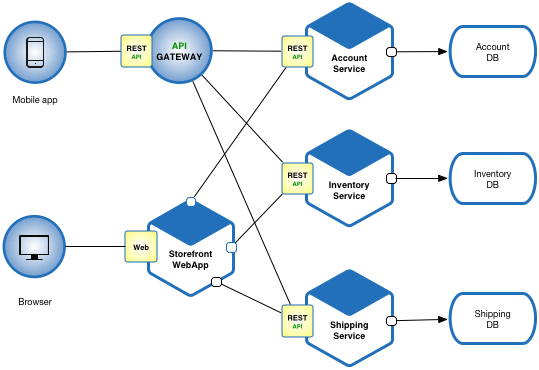
\includegraphics[width=0.7\textwidth]{Chapters/2-Grundlagen/Graphics/Microservice_Architecture.png}
  \caption{Beispielhafter Aufbau einer Micro-Service Architektur \cite{chris_richardson_microservices_nodate}}
  \label{fig:microservices}
\end{figure}
Entwickler verschiedener Micro-Services benutzen die Schnittstellen der jeweils Anderen, um Datenflüsse abzubilden, die zur Umsetzung des eigenen Micro-Service vonnöten sind. Gleichzeitig stellen sie für andere Micro-Services dem von ihnen entwickelten Micro-Service ebenfalls eine Schnittstelle bereit. 

In der Theorie ist für einen Service \textit{A} ist nicht von Bedeutung, wie ein anderer Service \textit{B} seine Funktionalität realisiert. Seine Schnittstelle und deren Definition ist \textit{A} bekannt. \textit{A} benutzt die Schnittstelle von \textit{B} beispielsweise, um Daten abzufragen, die zur Berechnung einer hypothetischen Funktion $F_A$ benötigt werden. Micro-Service \textit{A} stellt $F_A$ wiederum über eine Schnittstelle nach außen hin zur Verfügung. Die Nutzung einer Schnittstellenfunktion eines Micro-Service erfolgt entweder programmatisch durch den Zugriff eines anderen Micro-Service, oder über Anknüpfung an eine grafische Benutzeroberfläche.
\\

\paragraph{API-Versionen}\mbox{}\\

Diese Kapselung ermöglicht eine einwandfreie, getrennte Weiterentwicklung spezifischer Micro-Services, sofern sich die Schnittstellendefinition verschiedener Versionen nicht unterscheidet. Eine vollständige Äquivalenz zwischen den Schnittstellen verschiedener Micro-Service-Versionen kann jedoch nicht immer gewährleistet werden. 

Zur Lösung dieser Problematik schlägt \textit{Jean-Jacques Dubray} [TODO:Quelle] verschiedene Lösungsansätze vor. Eine Möglichkeit zum Design von Schnittstellen und deren Versionen ist das sogenannte ''Knoten-Modell''. In ihm sind benutzende Micro-Services $B_1, ..., B_n$ einer Schnittstelle \textit{S} fest an ihre Version gebunden. Sie besitzen keinerlei Garantie über die Äquivalenz der Schnittstelle in kommenden Versionen. Ändert sich die Schnittstelle, müssen alle von ihr abhängigen Benutzer ebenfalls manuell überprüft und geändert werden. 
\\
Eine weitere Strategie ist die sogenannte \textit{Punkt-zu-Punkt}-Methode. Ähnlich zum Knoten-Modell sind alle Benutzer einer bestimmten Schnittstelle zunächst an eine bestimmte Version gebunden. Im Gegensatz zum Knoten-Modell bleiben Micro-Services mit veralteten Schnittstellenversionen bei deren Änderung jedoch bestehen. Die Teilnehmer eines vorhandenen Netzes von miteinander verbundenen Micro-Services müssen also nicht sofort auf eine neue Version eingestellt werden. Einzelne Netzteilnehmer können bei Bedarf auf die neue Schnittstellenversion ihrer Partner aktualisiert werden. Die Micro-Services unterschiedlicher Schnittstellenversionen werden dabei parallel betrieben, damit der Zugriff auf veraltete Versionen dauerhaft gewährleistet werden kann.
\\
Die letzte von Dubray vorgeschlagene Lösungstrategie beschreibt das Modell einer ''kompatiblen Versionierung''. Anstelle einer festen Verbindung unterschiedlicher Benutzer an die Schnittstelle einer bestimmten Version sind letztere hier an alle Endpunkte der Schnittstellendefinition gebunden, die zu einem bestimmten Versionszeitpunkt verfügbar waren. Alle Folgeversionen müssen die Idempotenz der Funktionalität dieser Endpunkte hinsichtlich der vorangegangenen Versionen gewährleisten. Um einer Schnittstelle neue Funktionalität hinzuzufügen stellt man deswegen gänzlich neue Endpunkte zur Verfügung. Man spricht konkret von der ''Abwärtskompatibilität'' neuerer Schnittstellenversionen.

\paragraph{Kommunikation unter Micro-Services}\label{grundlagen:microcomms}
\mbox{}\\

Zum Datenaustausch bedienen sich Micro-Services verschiedener Netzwerkkommunikationsmodelle. Dabei unterscheidet man zwischen \textit{interner} oder \textit{horizontaler} und \textit{externer} beziehungsweise \textit{vertikaler} Kommunikation. Während erstere die Kommunikation zwischen Micro-Services einer Gruppierung von Micro-Services beschreibt, stellt letztere den Informationsaustausch zwischen einer solchen Gruppierung und externen Dienstleistern oder Nutzern dar. Eine Möglichzeit zur Umsetzung dieses Modells findet sich in Kapitel [TODO Kubernetes]. \\
Zum konkreten Datenaustausch bedienen sich Micro-Services dem ''Client-Servier'' Modell. Den Kommunikationspartnern steht dabei unter anderem das ''Request-Response''-Modell zur Verfügung [TODO: Grafik]. Ein Microservice \textit{A}, der Daten oder Funktionen bereitstellt, setzt diesen Vorgang über einen Server um. Dieser Server besitzt eine feste Adresse. Er stellt spezifische Datensätze oder Funktionen über einen oder mehrere, festgelegte Endpunkte bereit. Ein Client ist in der Lage, durch die Kombination einer Serveradresse und eines Endpunkt Anfragen nach diesen Daten oder der Ausführung einer Funktion zu stellen(\textit{Request}). Aufgabe des Servers ist es danach, eine sinnvolle Antwort an den Client zurückzusenden (\textit{Response}). Um den Abrufungsprozess weiterhin zu steuern, besitzt ein Client die Möglichkeit, seinen Anfragen bestimmte Parameter hinzuzufügen.
\textit{A}s Schnittstelle $S_A$ setzt sich im ''Response-Request-Modell'' aus allen Endpunkten zusammen, die \textit{A} über seinen Server nach außen hin verfügbar macht. $S_A$ legt weiterhin fest, ob und welche Parameter sowie deren Aufbau ein in ihr enthaltener Endpunkt besitzt. \\
Eine weitere Möglichkeit zum Datenaustausch bietet das ''Publisher-Subscriber-Modell''. In diesem benutzt der Micro-Service \textit{P}, der Daten bereitstellt, einen sogenannten ''Message-Broker''. Dieser Message-Broker stellt eine Art Kanal (\textit{Topic)} zur Verfügung, in welchen \textit{P} Daten oder Nachrichten zur Verfügung stellt. Diesen Vorgang nennt man ''Publishing''. Eine beliebige Anzahl an weiteren Micro-Services $S_0, ..., S_n$ ist in der Lage, sich beim Message-Broker für diese Topic zu registrieren. Wenn \textit{P} eine Nachricht in diesen Kanal hinterlegt, werden alle registrierten Services $S_0,...,S_n$ benachrichtigt. Diese sind dann in der Lage, die so gewonnenen Daten weiterzuverarbeiten.  

- Datenformate

\subsection{Container}

Ein \textit{Container} ist eine Einheit, welche Software, ihre Abhängigkeiten sowie Konfigurationen in sich bündelt. Er wird wiederum innerhalb eines \textit{Container-Abbildes} gebündelt. Ein Container-Abbild ist eine Art Vorlage, die den Erstellungsprozess eines Containers beschreibt. Es enthält weiterhin zusätzliche Informationen, die zur Ausführung der im Container enthaltenen Software benötigt werden. Unter diesen befinden sich unter anderem verschiedene Systemtools und -bibleotheken, sowie eine Laufzeitumgebung. Während Micro-Services die Funktionen einer Cloud-Native-Architektur einzeln realisieren, kapseln Container einzelne Micro-Services wiederum vom Betriebssystem ihres ausführenden Computers ab. Da Container-Abbilder alle nötigen Informationen zur Ausführung von Software beinhalten, können in ihnen gekapselte Micro-Services betriebssystemunabhängig ausgeführt werden, solange auf dem ausführenden System eine sogenannte \textit{Engine} existiert, welche eine Brücke zwischen seinem Betriebssystem und dem Container liefert. Container sind durch diesen Vorgang vom ausführenden System und anderen Containern isoliert. Möchte Software innerhalb eines Container in ihm beinhaltete Daten oder Abhängigkeiten verändern, geschieht das durch die sogenannte ''Copy-on-Write''-Strategy (COW). Die zu verändernden Daten werden zunächst kopiert, bevor sie verändert werden. Je nach Implementierung liefern verschiedene Container-Architekturen unterschiedliche Strategien, um veränderte Daten nachhaltig zu persistieren. In der Micro-Service-Architektur werden diese Stragien in der Regel selten benötigt, da ihre Bestandteile meist zustandslos sind. Durch die in diesem Abschnitt vorgestellten Methoden sind Container in der Lage, ihre Funktion unabhängig der zugrunde liegenden Infrastruktur auszuführen. \cite{docker_what_nodate}. 

\subsection{Service-Meshes}
Um die Vorteile und Eigenschaften eines Service-Meshes zu betrachten, muss zunächst der Begriff Container-Orchestration beleuchtet werden.
\subsubsection{Container-Orchestration}
Werden die Services einer Micro-Service-Architektur in Containern betrieben, können sie unabhängig von einer festen Infrastruktur betrieben werden.\\
Für eine Cloud-Native Architektur ist dies von Vorteil. Denn Container lassen sich mit minimaler Verzögerung starten und stoppen. Zudem können wir horizontal skalieren, indem wir weitere Container starten. Allerdings ergeben sich dadurch einige Probleme. Zunächst ein Mal müssten Container automatisch gestartet, gestoppt und neu gestartet werden. Die Skalierung des Systems, oder im Fehlerfall das Neu starten von Containern darf keine menschliches Aufgabe sein. Denn dies wäre zwangsläufig mit einer zu großen Verzögerung verbunden.\\
Um diese Verzögerung weiter zu reduzieren, könnten bereits Ersatz-Container vorgehalten werden. Im Fehlerfall oder für die Skalierung würde ein Umleiten des Traffics genügen. Dies erfordert ein automatisiertes Load-Balancing.\\
Ein funktionierendes Load-Balancing ist auch für die Container zu Container Kommunikation notwendig. Wird ein Service durch mehrere Container umgesetzt, gilt es zu definieren, welcher dieser Container adressiert werden soll. Dieses Problem wird als internal Load-Balancing bezeichnet. \\\\

Die\textit{ Container Orchestration}\cite{scholl_cloud_2019} behebt diese Probleme. Der \textit{Container-Orchestrator} liegt als eine Schicht über den Containern. Er ist verantwortlich für das starten und stoppen von Containern. Außerdem teilt er flexibel Rechenleistung zu und skaliert das System passend zum bestehenden Traffic.\\
Stehen mehrere Server zur Verfügung, platziert er neue Container auf den Servern mit der niedrigsten Auslastung. Außerdem verschiebt er Container, sollte die Auslastung zunehmen. Auch andere Metriken sind für die Server Auswahl und die Verschiebung der Container möglich.\\
Der Container-Orchestrator überwacht zudem die Gesundheit der Container. Falls nötig startet er diese neu.\\
Abschließend ist er für das interne und externe Load-Balancing verantwortlich. Realisieren mehrere Container den selben Service, leitet der Load-Balancer den Traffic zu dem geeignetsten Container weiter. \\
Neben den genannten Funktionen kann der Container-Orchestrator auch für das State-Management und viele weitere Aspekte des Systems zuständig sein.\\
Scholl et Al.\cite{scholl_cloud_2019} sieht in Google Kubernetes \cite{kubernetes_production-grade_nodate} die populärste Container Orchestrator Wahl.
\subsubsection{Herausforderungen der Micro-Service-Architektur}
Durch die Aufteilung unserer Anwendung in Micro-Services haben wir die Komplexität der einzelnen Bestandteile unserer Architektur reduziert. Man sollte allerdings bedenken, dass gleichzeitig die Komplexität auf dem System-Level zugenommen hat. Jeder Service einer Micro-Service Architektur wird, neben der Business Logik, unter anderem folgendes enthalten \cite{codingwithnana_istio_nodate}:
\begin{itemize}
    \item Jede Service wird eine Retry-Logik umsetzen. Es ist möglich, dass Services nicht erreichbar sind. Ist dies der Fall, muss definiert werden, wie oft eine Verbindungsversuch unternommen wird. Ferner ist eine Ausnahmebehandlung zu ergänzen.
    \item Darüber hinaus ist die Umsetzung der Sicherheit zu beachten. Eine Firewall kann die Anwendung von außen Schützen. Allerdings gilt es das Konzept der in-depth Security umzusetzen. Diese verlangt, dass auch die Kommunikation unter den Containern abgesichert ist. Ferner sollte nicht jeder Container frei mit jedem anderen Container kommunizieren dürfen.
    \item Abschließend ist für die Automatisierung einer Überwachung unumgänglich. Es gilt Metriken zu erfassen und auf Basis dessen zu Handeln. Logger und Logik zum Fehlerfinden müssen ebenfalls in jedem Service integriert werden.
\end{itemize}
Ein Vorteil der Microservice-Architektur war es, dass jedes Team einen klar getrennten Anteil der Anwendung entwickelt. Allerdings muss jedes Team, neben der eigentlichen Business Logik, die zuvor genannten Funktionen entwickeln, verwalten und konfigurieren. Diese Konfiguration kann nicht individuell für jeden Service statt finden, ohne zu Fehlern und Problem zu führen. Außerdem wird die Fehlersuche deutlich erschwert. Eine Isolation von Fehlern in einem einzigen Service ist nicht mehr sichergestellt.

\subsubsection{Vorgehensweise von Service-Meshes}
\textit{Service Meshes} nutzen einen sogenannten \textit{Sidecar-Proxy} \cite{codingwithnana_istio_nodate}. Dieser wird in Abbildung \ref{fig:service-mesh} dargestellt. Jedem Container wird ein weiterer Container hinzugefügt. Dieser fungiert als Proxy. Er nimmt demnach Verbindungen an und leitet sie zu dem eigentlichen Service weiter. Diese Side-Car-Proxys werden durch die \textit{Control-Plane} verwaltet und in die einzelnen Services injiziert. Ein neuer Service muss demnach die zuvor genannten Probleme, wie Sicherheit oder die Retry-Logic nicht erneut umsetzen. Außerdem ist die Control-Plane eine zentrale Schnittstelle um die gesamte Anwendung zu konfigurieren und zu Überwachen. Neben den genannten Funktionen, kann ein Service-Mesh auch weitere Aspekte, wie zum Beispiel das Load-Balancing, lösen. Meist wird an dieser stelle aber auf einem Container-Orchestrator wie Kubernetes \cite{kubernetes_production-grade_nodate} aufgebaut. Eine mögliches Service-Mesh wäre zum Beispiel Istio \cite{istio_istio_nodate}. 
\begin{figure}[bth] 
  \centering
  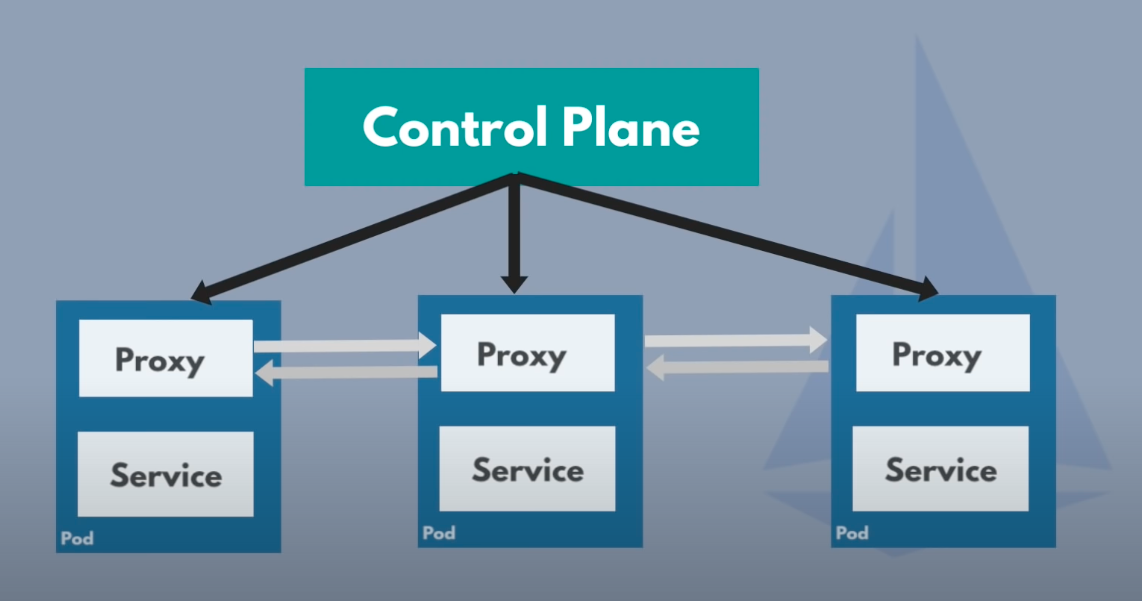
\includegraphics[width=0.7\textwidth]{Chapters/2-Grundlagen/Graphics/service-meshes.png}
  \caption{Service-Meshes am Beispiel Istio \cite{codingwithnana_istio_nodate}}
  \label{fig:service-mesh}
\end{figure}

\subsection{Organisation}

Organisation, CI/CD und DevOps

- In der Praixs ein Repo pro Service
- Konfigurationen über Environment
- Dependencies über Package Manager
- 


%Analyse
\cleardoublepage%=========================================
% 	   Analyse     		 =
%=========================================
\chapter{Analyse}
\label{ch:analyse}

\section{Differenzierung}

Dieses Kapitel vergleicht die Prinzipien, Eigenschaften und Umsetzungskriterien der Cloud-Native-Architektur mit denen anderer Architekturen und stellt deren Unterschiede dar.

\subsection{Monolithen}

Ein grundlegender Unterschied zwischen einer monolitischen Softwarearchitektur und der einer Cloud-Native-Architektur findet sich in der Zusammensetzung ihrer Komponenten. Ein sogenannter \textit{Monolith} ist ein einheitliches Softwaresystem, welches die gesamte Programmlogik, Datenverwaltung und die Benutzeroberfläche in einer abgeschlossenen, ausführbaren Datei verbindet. Die in ihr enthaltenen Komponenten sind oft eng miteinander verknüpft. Diese Zusammensetzung bietet einen in den Anfangsphasen der Entwicklung simplen Implemtierungsprozess, da die Entwickler während der Umsetzung eines Prototyps unmittelbar Änderungen an den verschiedenen Komponenten umsetzen können. In den Anfängen eines Projektes ist es zudem simpel, Änderung zu veröffentlichen. Dazu muss lediglich eine neue Version der gebündelten Datei des Monoliths an seine Nutzer verteilt werden.

Ein zunehmendes Wachstum des Monoliths fördert jedoch eventuell einige, nicht unerhebliche Nachteile. Erhöht sich die Größe des Monoliths und seiner Codebasis, wächst die Wahrscheinlichkeit von abnehmender modularität seiner Bestandteile. Wenn sie stark miteinander verwoben sind, steigt die Komplexität bei notwendigen Veränderungen oder der Einführung neuer Funktionen an. Gleichzeitig wächst die Einarbeitungszeit in das Projekt für neue Teammitglieder. Es besteht weiterhin die Möglichkeit, dass sich der Softwaremonolith in einen ''Big Ball of Mud'' verwandelt. ''Ein Big Ball of Mud ist ein planlos strukturierter, ausufernder, schlampiger, mit Klebeband und Bindedraht zusammengehaltener Spaghetti-Code-Dschungel [todo: CITE].'' Mit zunehmender Seniorität der Mitglieder des Entwicklungsteams besteht außerdem die Gefahr, dass nur wenige oder gar keine Entwickler die gesamte Funktion des Monolithen vollständig nachvollziehen können. Schlussendlich ist man in der Entwicklung eines Monoliths meist unabdinglich an seine ursprünglich ausgewählte Technologieplatform gebunden. Der dichte Verbund der Komponenten des Monoliths erschwert den Austausch einzelner Technologien erheblich. \\

Der Aufbau eines Cloud-Native-Softwareprojektes steht im direkten Gegensatz zur monolitischen Softwarearchitektur. Es besteht aus individuellen, lose gekoppelten Kleinstbausteinen. Ihre Berührungspunkte untereinander bestehen einzig und allein aus ihren nach außen hin verfügbaren Schnittstellen. Aufgrund dieser Tatsache ist die Modurarität und Abgeschlossenheit der Bestandteile dauerhaft gewährleistet. Weiterhin ermöglicht die Kapselung der verschiedenen Micro-Services eine programmiersprachenagnostische Entwicklung und somit die Auswahl des ''Best Tool For The Job''. \\ 
Die Komplexität der Bestandteile eines Cloud-Native-Softwaresystems besteht im Gegensatz zu denen eines Monolithen nur aus der Komplexität der einzelnen Micro-Services. Da die Schnittstellen der verschiedenen Micro-Services fest definiert sind, kann bei der Betrachtung eines einzelnen Micro-Services die interne Funktionsweise seiner Interaktionspartner gänzlich außer Acht gelassen werden. Im Idealfall wird ein Micro-Service außerdem von genau einer festen Gruppe oder eines festen Teams von Entwickler verwaltet. Deren Mitglieder benötigen dann nur das Wissen über die Funktionalität des von ihnen betreuten Bestandteils der gesamten Architektur. Diese Tatsachen erleichtern den Entwicklungsprozess bei Fehlerbehebungen, der Erweiterung eines Micro-Service um zusätzliche Funktionen und das Testen der unterschiedlichen Micro-Services als abgeschlossene Einheit. Im konkreten Testprozess eines einzelnen Micro-Service kann die Funktion anderer, zum Funktionsaufruf benötigter Micro-Services durch den Programmierer simuliert werden. Diese Aufteilung hat jedoch den Nachteil, dass die Komplexität des Gesamtsystems direkt im Zusammenhang zur Anzahl und Qualität der Dokumentation seiner Einzelteile steht. Je größer die Anzahl unterschliedlicher Micro-Services, desto schwieriger ist es für die Beauftragten des Softwaresystemes, einen Überblick zu behalten. Bei sehr großen Systemen steigt die Gefahr von Quelltextduplizierung und vermindeter Auffindbarkeit bereits existierender Micro-Services, die eine benötigte Funktionsweise bereits abdecken. \\
Solange sich die Schnittstellen der Micro-Services nicht ändern, kann die Weiterentwicklung unabhängig von anderen Implementierungsteams geschehen. Strategien zur Anpassung des Gesamtsystems nach der Veränderung einer Schnittstelle finden sich in Kapitel \ref{grundlagen:microcomms}. Diese im vorangegangenen Absatz genannten Punkte lassen sich unter den Begriffen \textit{Agilität} und \textit{Continous Innovation} zusammenfassen. \\ 
Im Kontrast zur monolitischen Softwarearchitektur ermöglicht der Aufbau der Micro-Service-Architektur und die Bereitstellung von Micro-Services auf Cloud-Hostern einen dynamischen Austausch ihrer Bestandteile zum Zeitpunkt der Veröffentlichung neuer Versionen. Damit muss ein Benutzer des Softwaresystems bei Änderung seiner Komponenten nur selten in Kenntnis gesetzt werden. Dieser Prozess ermöglicht die Minimierung von Fragmentierungen zwischen den unterschiedlichen, aktiv genutzten Versionen eines Softwaresystems, da es weitestgehend automatisiert aktualisiert werden kann. Dieser Prozess wird mit dem Begriff \textit{Continous Delivery} bezeichnet. \\

Die Cloud-Native-Architektur unterscheidet sich von einer monolitischen weiterhin durch den Prozess der Skalierung. Der traditionelle Skalierungsansatz eines Monolitihen ist die parallele Ausführung mehrerer Instanzen und die subsequente Verteilung von Anfragen über einen ''Load-Balancer''. Da der Monolith jedoch ein festes Bündel seiner Bestandteile ist, ist es nur möglich, ihn als Ganzes zu skalieren. Die Aufteilung der Micro-Services der Cloud-Native-Architektur erlaubt es hingegen, jeder Komponente genau nur die benötigten Ressourcen zuzuweisen. [TODO: Caching?] Dieses Vorgehen erlaubt eine dynamische Umverteilung von bereits vorhandener Ressourcen und eine Zuweisung gänzlich neuer Rechen- und Speicherleistung bei veränderter Lastverteilung oder einer Welle von neuen Anfragen. Im Ideallfall werden solche Skalierungsprozesse vom verwendeten Cloud-Hoster vollautomatisiert umgesetzt. Ihre dynamische Natur erlaubt weiterhin flexible Bezahlungsmodelle. Im sogenannten ''Pay-As-You-Go''-Modell bezahlt ein Nutzer eines Cloud-Hosters nur genau die Ressourcen, die zur Ausführung seiner Software genutzt werden. Die Zustandslosigkeit der Bestandteile einer Cloud-Native-Architektur erlaubt eine Fokussierung auf die verwendeten \textit{Datastores} bei der Umsetzung effizienter Caching-Strategien. 


- Verfügbarkeit
 - Single Point of Failure

\section{Zusammenfassung}

%Konzeption
\cleardoublepage%=========================================
% 	   Tools     		 =
%=========================================
\chapter{Tools und Industriestandards}
\label{ch:tools}
In diesem Kapitel werden die Tools und Industriestandards betrachtet, welche für das Umsetzen der in Kapitel 2.4 vorgestellten Cloud-Native Technologien zum Einsatz kommen. In der Praxis gibt es viele verschiedene Projekte und Ansätze, Container sowie Container-Orchestrator zu realisieren, die jeweils eigene Vor- und Nachteile mit sich bringen. Zusätzlich existiert heutzutage eine Vielzahl an Cloud-Anbietern, welche ihre Hardwareressourcen für das Aufsetzen von Cloud-Native Anwendungen zur Verfügung stellen und dazu diverse Dienste für das einfachere Betreiben dieser anbieten.
\\\\
Im Folgenden werden die am häufigsten verwendeten Tools und Industriestandards vorgestellt und anschließend ein Überblick darüber verschafft, in welchen Industrien und Branchen Cloud-Native Anwendungen eingesetzt werden.

\section{Container Runtime Environments}
Von Vielen wird der Begriff „Container“ schnell mit Docker assoziiert. Hierbei handelt es sich jedoch bei weitem nicht um das einzige Projekt, welches das Konzept der Containervirtualisierung realisiert. Neben dieser wohl bekanntesten Container Runtime von Docker Inc. gibt es eine Vielzahl an weiteren Tools, welche ebenfalls die Möglichkeit bieten, Applikationen in Containern zu isolieren.
\\\\
Bevor wir die verschiedenen Container Runtimes genauer betrachten, muss zunächst definiert werden, was man unter einer Container Runtime versteht.

\subsection{Container Runtime}
Eine Container Runtime hat Ähnlichkeiten zu der Runtime einer gewöhnlichen Software-Applikation. Es handelt sich hierbei um Software, welche die einzelnen Komponenten, die für das Starten eines Containers benötigt werden, verwaltet und dafür sorgt, dass diese funktionsfähig sind \cite{evan_baker_comprehensive_2021}. Sie ermöglicht, dass der Nutzer sich nicht selbst um das Management dieser Komponenten kümmern muss, wodurch das Arbeiten mit Containern und deren Deployment effizienter durchgeführt werden können.

\subsection{Linux Control Groups (cgroups)}
Im Jahr 2007 wurden in den Linux Kernel sogenannte cgroups (Linux Control Groups) integriert \cite{evan_baker_comprehensive_2021}. Hierbei handelt es sich um ein Linux Kernel Feature, welches ermöglicht, Prozesse in hierarchischen Gruppen zu organisieren, deren Nutzung von verschiedenen Ressourcen limitiert und überwacht werden kann \cite{noauthor_cgroups_2021}.\\
Auf Basis dieses neuen Features wurden anschließend einige erste Projekte ins Leben gerufen, welche containerisierte Prozesse ausführten konnten. Hierzu zählen unter anderem LXC, LMCTFY, systemd-nspawn oder rkt \cite{evan_baker_comprehensive_2021}.

\subsection{Linux Containers (LXC / LXD)}
LXC, kurz für Linux Containers, wurde kurz nach cgroups vorgestellt und befindet sich seit 2008 in Entwicklung \cite{noauthor_lxc_2021}. Das Projekt wurde hauptsächlich in C, Shell und Python geschrieben, und verwendet ein eigenes Containerformat namens Linux-Containers. Der Fokus von LXC liegt auf sogenannten Full-System-Containers \cite{noauthor_lxc_2021}. Hierbei handelt es sich um Container, die darauf abzielen, ein gesamtes Betriebssystem zu virtualisieren. Diese Art von Containern ist für Cloud-Anwendungen eher ungeeignet, da hier kein ganzes Betriebssystem virtualisiert werden muss, sondern lediglich ein einzelner Prozess abgekapselt ausgeführt werden soll.\\\\
LXC hat später mit LXD (Lexdi) noch ein Folgeprojekt erhalten, welches ebenfalls auf Full-System-Container spezialisiert ist. Letztendlich hat sich LXC aber, ebenso wie der Ansatz von systemd, systemd-nspawn, nie bei den Endnutzern durchgesetzt. Sie wurden jedoch von anderen Systemen verwendet. Docker wurde beispielsweise teilweise auf Basis von LXC gebaut \cite{evan_baker_comprehensive_2021}.

\subsection{LMCTFY (Let Me Contain That For You)}
LMCTFY (Let Me Contain That For You) war ein frühes Container-Projekt von Google, welches zum Großteil in C++ geschrieben ist. Der Fokus lag hierbei darauf, ähnlich wie bei Docker, einzelne Applikationen innerhalb eines Containers isoliert auszuführen. Das Projekt ist Open Source, wurde jedoch eingestellt als Docker zunehmend an Popularität gewann \cite{noauthor_lmctfy_2021}.

\subsection{Docker}
Docker ist wohl das bekannteste Projekt für Containervirtualisierung. Es wurde zu Beginn unter dem Namen dotCloud entwickelt und verwendete zunächst LXC als Basis. Nach kurzer Zeit gründete Docker zusammen mit einigen anderen Unternehmen die Open Container Initiative (OCI), um einige Standards für Containertechnologien zu definieren, worauf hin LXC durch eine eigens entwickelte Schnittstelle namens libcontainer ersetzt wurde \cite{evan_baker_comprehensive_2021}.
\\\\
Docker wird von vielen mit dem Begriff Containervirtualisierung gleichgesetzt und bietet neben einer Container Runtime viele weitere Features. Die hauseigene Container Runtime unterstützt Container in einem eigens von Docker entwickelten Format (Docker-Container). Das Tool ist in Go geschrieben und wird von Docker Inc. entwickelt. Docker unterstützt keine Full-System-Container und fokussiert sich auf die Isolierung einzelner Applikationen, wodurch es für die Verwendung bei Microservices und Cloud-Native-Architekturen geeignet ist.
\\\\
Das Docker-Tool beinhaltet neben dem Starten eines Containers viele weitere Features, wie beispielsweise das automatische Erstellen von Images, auf dessen Basis dann ein Container erstellt werden kann, oder das Hochladen eines solchen Images in das sogenannte Docker Hub. Hierbei handelt es sich um eine große Sammlung von Docker-Images, welche gratis verwendet werden können. Fast alle großen IT-Projekte, wie beispielsweise bekannte Datenbanken wie MySQL oder Redis, sind hier mit einem Docker-Image vertreten \cite{noauthor_dockerhub_2021}. Mit Hilfe des Docker-Tools kann man durch ein einfaches Ausführen von „docker run“ auf das jeweilige Image sofort einen Container auf dessen Basis erstellen, wobei Docker alle benötigten Abhängigkeiten automatisch herunterlädt. Somit können all diese Tools ohne eine komplizierte Installation sofort verwendet werden. Als Nutzer hat man zusätzlich die Möglichkeit, seine eigenen Images gratis auf Docker Hub hochzuladen, in private oder öffentliche Registries. Auf öffentliche Registries haben dann auch andere Nutzer Zugriff und können diese Images verwenden. Dabei bietet Docker Hub zusätzlich eine Versionierung von Images, indem diese mit einem Versions-Tag versehen werden können.
\\\\
Des Weiteren bietet Docker mit Docker-Compose ein Tool zum Starten von mehreren Containern gleichzeitig, wobei Abhängigkeiten und Verbindungen zwischen diesen realisiert und berücksichtigt werden können. Zusätzlich gibt es mit Docker Swarm ein hauseigenes Orchestrierungs-Tool. Docker ist somit ein leicht zu bedienendes All-In-One Werkzeug für Containervirtualisierung.
\\\\
Diese Einfachheit hat stark zu der heutigen Beliebtheit von Docker beigetragen. Außerdem wird Docker von vielen Cloud-Anbietern und Container-Orchestratoren unterstützt.

\subsection{rkt („Rocket“)}
Mit rkt („Rocket“) wurde von den Entwicklern der Linux Distribution CoreOS eine Alternative für Docker entwickelt. Auch hier wurde als Programmiersprache Go verwendet \cite{noauthor_rkt_2021}. Zur damaligen Zeit enthielt rkt einige Features, welche Docker und anderen Container Runtimes überlegen waren. Beispielsweise war es bei rkt nicht notwendig, alle Prozesse als root zu starten \cite{evan_baker_comprehensive_2021}. Außerdem unterstützt rkt neben ihrem eigenen Containerformat auch weitere Formate, unter anderem Docker-Container.
\\\\
CoreOS hat zunächst mit appc einen eigenen Container-Standard veröffentlicht, hat sich jedoch später bei der Gründung der Open Container Initiative dieser als Gründungsmitglied angeschlossen \cite{evan_baker_comprehensive_2021}. Daraufhin war rkt eine Zeit lang der größte Konkurrent von Docker. Nachdem letzteres jedoch immer mehr an Popularität gewann, wurde rkt letztendlich 2020 eingestellt und wird aktuell nicht mehr aktiv weiterentwickelt \cite{noauthor_rkt_2021}.

\subsection{Podman}
Podman steht für Pod Manager und ist eine von Redhat entwickelte Docker Alternative. Der Fokus liegt hierbei, wie der Name bereits andeutet, auf sogenannten Pods. Hierbei handelt es sich um eine Abstraktion über einem Container oder mehreren Containern, die sich gewisse Ressourcen teilen. Der Begriff stammt aus dem Kubernetes-Umfeld.
\\\\
Podman ist in Go geschrieben \cite{noauthor_podman_2021}. Redhat kritisiert an Docker, dass es mit der Docker Engine ein All-In-One-Tool für Containervirtualisierung bietet. Man möchte mit Podman die UNIX-Philosophie verfolgen, welche besagt, dass ein Programm immer eine Aufgabe erledigen soll. Somit wird Podman nur für das Starten und Managen von Containern bzw. Pods verwendet, nicht aber beispielsweise für das Bauen von Images. Hierfür gibt es wiederum ein eigenes Tool, welches sich darauf spezialisiert, wie zum Beispiel buildah. \cite{evan_baker_comprehensive_2021}.

\subsection{Open Container Initiative Runtimes}
Wie bereits erwähnt haben sich einige Unternehmen zusammengeschlossen und die Open Container Initiative gegründet. Die hierbei entstandenen Spezifikationen beschreiben eine sogenannte Low-Level-Runtime. Dies bedeutet, die Runtimes fokussieren sich auf das Management des Lebenzyklus von Containern und müssen sich ansonsten um nichts weiteres kümmern \cite{evan_baker_comprehensive_2021}. Sie werden somit meist nicht vom End-User direkt verwendet, sondern sind in eine andere High-Level-Container-Software, wie beispielsweise Docker, eingebettet.
\\\\
Die bekannteste Low-Level-Runtime ist runC. Hierbei handelt es sich um die OCI Runtime von Docker, welche im Rahmen von libcontainer entstanden ist. Das Projekt ist in Go geschrieben und Open Source verfügbar \cite{evan_baker_comprehensive_2021}.
\\\\
Oracle hatte mit Railcar eine Alternative zu runC ins Leben gerufen, welche ebenfalls auf die Spezifikationen der OCI aufsetzt. Als Programmiersprache wurde Rust gewählt, welche sich ebenso wie Go als sehr geeignet für Containervirtualisierung herausstellte. Trotzdem wurde das Projekt später eingestellt \cite{evan_baker_comprehensive_2021}.

\subsection{Open Container Initiative Runtimes}
Wie bereits erwähnt haben sich einige Unternehmen zusammengeschlossen und die Open Container Initiative gegründet. Die hierbei entstandenen Spezifikationen beschreiben eine sogenannte Low-Level-Runtime. Dies bedeutet, die Runtimes fokussieren sich auf das Management des Lebenzyklus von Containern und müssen sich ansonsten um nichts weiteres kümmern \cite{evan_baker_comprehensive_2021}. Sie werden somit meist nicht vom End-User direkt verwendet, sondern sind in eine andere High-Level-Container-Software, wie beispielsweise Docker, eingebettet.
\\\\
Die bekannteste Low-Level-Runtime ist runC. Hierbei handelt es sich um die OCI Runtime von Docker, welche im Rahmen von libcontainer entstanden ist. Das Projekt ist in Go geschrieben und Open Source verfügbar \cite{evan_baker_comprehensive_2021}.
\\\\
Oracle hatte mit Railcar eine Alternative zu runC ins Leben gerufen, welche ebenfalls auf die Spezifikationen der OCI aufsetzt. Als Programmiersprache wurde Rust gewählt, welche sich ebenso wie Go als sehr geeignet für Containervirtualisierung herausstellte. Trotzdem wurde das Projekt später eingestellt \cite{evan_baker_comprehensive_2021}.
\\\\
Auch Redhat hat eine eigene Implementation der OCI Spezifikationen entwickelt. Die Runtime heißt crun und wurde in C geschrieben. Laut dem offiziellen GitHub Repository ist crun schneller als runC und benötigt weniger Ressourcen. Man hat sich bewusst für C als Programmiersprache entschieden, da C leichtgewichtiger als Go ist und die in Go geschrieben Runtimes meist selbst auf C-Module zugreifen, um ihre Container zu starten \cite{noauthor_crun_2021}.

\subsection{Kubernetes Container Runtime Interface (CRI)}
Kubernetes hat als bekanntester Container Orchestrator mit dem Release von Kubernetes 1.5 das Container Runtime Interface eingeführt. Hierbei handelt es sich um ein Plugin-Interface, welches Kubernetes ermöglicht verschiedene Container-Runtimes zu verwenden, indem sie dieses Interface implementieren \cite{noauthor_cri_2021}. Das CRI erweitert die von der OCI definierten Spezifikationen um einige für die Orchestrierung relevanten Funktionalitäten.
\\\\
Eine Implementation des CRI ist containerd. Es handelt sich dabei um die High-Level-Runtime von Docker, welche als Low-Level-Runtime standardmäßig runC verwendet \cite{evan_baker_comprehensive_2021}. Das Projekt wurde wie Docker in Go geschrieben und unter einer Open-Source Lizens losgelöst von Docker auf GitHub veröffentlicht \cite{noauthor_containerd_2021}.
\\\\
Mit CRI-O hat auch Redhat eine Implementation des CRI veröffentlicht. CRI-O soll als Brücke zwischen dem CRI und OCI Runtimes fungieren und ermöglicht das Einbinden von allen OCI Runtimes in Kubernetes und ist dabei leichtgewichtiger als Docker \cite{noauthor_cri-o_2021}.

\section{Container Orchestrator}
Auch für die Container Orchestrierung gibt es einige verschiedene Produkte auf dem Markt. Das bereits erwähnte Kubernetes ist das am häufigsten eingesetzte Tool und hat sich mittlerweile als Industriestandard durchgesetzt. Es existieren jedoch noch weitere Projekte, von denen einige in diesem Kapitel vorgestellt werden.

\subsection{Kubernetes}
Kubernetes ist ein Open-Source Container-Orchestrator. Das Projekt wurde von Google entwickelt und 2014 erstmals veröffentlicht \cite{noauthor_kubernetes_2021}. Wie bei Docker wurde auch hier Go als Programmiersprache gewählt. Oftmals wird Kubernetes mit k8s abgekürzt, wobei die “8” hierbei für die Anzahl der Buchstaben zwischen “K” und “s” steht.
\\\\
Kubernetes hat sich mit der Zeit gegen andere Container Orchestrator durchgesetzt und wird aktuell als der Standard für Container-Orchestration angesehen. Wie bereits erwähnt wurde ein eigenes Container Runtime Interface (CRI) definiert, durch welches Kubernetes alle größeren Container Runtimes unterstützt. Außerdem haben alle großen Cloud-Anbieter wie Amazon oder Google Kubernetes-Support. Oftmals bieten diese auch eigene sogenannte Managed Kubernetes Services an. Hierbei handelt es sich um von den Cloud-Anbietern eigens entwickelte Schnittstellen für das Arbeiten mit Kubernetes, welche dieses oftmals erleichtern und für die jeweilige Cloud-Plattform zugeschnitten sind.

\subsection{Docker Swarm}
Docker beinhaltet mit Docker Swarm, oftmals auch als Swarm Mode bezeichnet, ein hauseigenes Orchestrierungstool. Es ist Teil der Docker Engine und ist direkt in die Docker CLI eingebunden. Man benötigt somit keine zusätzliche Orchestrierungssoftware, wenn man bereits Docker installiert hat \cite{noauthor_dockerswarm_2021}.
\\\\
Docker Swarm ist verglichen mit Kubernetes deutlich einfacher zu bedienen. Kubernetes ist viel komplexer und bietet mehr Konfigurationsmöglichkeiten. Trotzdem sind die Grundfunktionalitäten eines Container Orchestrators alle in Docker Swarm enthalten. Docker bietet somit einen leicht zu bedienden Container Orchestrator und vereinfacht die Orchetration für den Nutzer, wenn die Komplexität von Kubernetes nicht benötigt wird. Docker Swarm beinhaltet beispielsweise von Haus aus kein Monitoring seiner Services., während Kubernetes dies automatisch macht. Außerdem ist Docker Swarm ist nur mit Docker-Containern kompatibel, wobei Kubernetes neben Docker auch andere Container-Formate untersützt.

\subsection{Docker Compose}
Docker bietet neben dem Swarm Mode mit Docker Compose ein weiteres Tool, über welches man Applikationen bestehend aus mehreren Containern realisieren kann. Hierbei handelt es sich aber nicht um eine vollwertigen Container Orchestrator. Man kann mit Docker Compose mehrere Container über ein virtuelles Netzwerk miteinander verbinden und diese somit miteinander kommunizieren lassen. Es ist aber keine Verteilung auf mehrere Nodes möglich. Dafür ist die Konfiguration von Docker Compose sehr einfach. Es eignet sich somit beispielsweise für das lokale Testen einer Cloud Anwendung.

\subsection{Fleet}
Fleet ist ein ehemaliges Projekt von CoreOS. Es wurde in Go entwickelt und unter einer Open Source Lizenz veröffentlicht \cite{noauthor_fleet_2021}. Fleet basiert auf systemd und etcd, einem Key-Value-Store für verteilte Systeme \cite{noauthor_etcd_2021}. Mittlerweile wurde das Projekt eingestellt und CoreOS empfiehlt Kubernetes als Container Orchestrator \cite{noauthor_fleet_2021}.

\subsection{Apache Mesos}
Apache Mesos ist ein Open Source Cluster-Manager. Im Gegensatz zu den anderen Orchestratoren kann Apache Mesos nicht nur Container orchestrieren, sondern kann generell für das Verwalten von Anwendungen auf einem Cluster eingesetzt werden. Das Framework Marathon ist Teil von Apache Mesos und ist für die Container-Orchestration zuständig. Marathon ist in Scala geschrieben und bietet eine REST-Schnittstelle, über welche das Cluster verwaltet werden kann \cite{noauthor_marathon_2021}. Es werden Container in einem eigenen Mesos-Container-Format sowie Docker-Container unterstützt \cite{noauthor_mesosphere_2021}.

\section{Managed Kubernetes Services}
...
\section{Nutzung in der Industrie}
...



%Implementierung
\cleardoublepage%=========================================
% 	   Fallstudie     		 =
%=========================================
\chapter{Fallstudie}
\label{ch:fallstudie}
In den vorherigen Kapiteln wurde auf das Architekturmuster Cloud-Native und dessen Eigenschaften eingegangen. Ferner wurden Technologien vorgestellt, welche bei der Umsetzung einer Cloud-Native-Architektur unterstützen. In diesem Kapitel wird eine Fallstudie betrachtet. Anschließend wird für die Fallstudie eine Cloud-Native Architektur vorgestellt und evaluiert.

\section{Vorstellung der Fallstudie}
\section{Anforderungen}
\section{Konzeption}
\section{Umsetzung}
\section{Evaluation}
Abschließend gilt es zu betrachten, auf welche Probleme wir während der Umsetzung gestoßen sind. Hier muss angemerkt werden, dass die Umsetzung in einem engen Zeitrahmen statt gefunden hat. Jedes der gezeigten Konzepte kann noch weiter ausgearbeitet werden. Ferner wird jedes der gezeigten Konzepte exponentiell komplexer, sollte die Anwendung in einer produktiven Umgebung eingesetzt werden. Einige dieser Konzepte werden in den folgenden Abschnitten erläutert. Zunächst gilt es allerdings zu analysieren, was unsere Anwendung bereits im aktuellen Zustand problemlos umsetzen kann.\\
\\
Im Kapitel Konzeption wurden die einzelnen Komponenten unser Anwendung gezeigt. Jede dieser Komponenten stellt ein eigenes Kubernetes Deployment dar. Dies ermöglicht es jede dieser Komponenten zu skalieren. Die Kommunikation der Komponenten untereinander ist weiterhin problemlos möglich. Ferner werden Nutzeranfragen auf die verschiedenen Instanzen der Benutzerschnittstellen verteilt. Von außen ist nicht ersichtlich, dass mehrere Instanzen der Komponenten betrieben werden. Unsere Anwendung könnte demnach auf einem Kubernetes Cluster betrieben werden. Stellt dieses genügen Rechen-Ressourcen bereit kann eine beliebige Anzahl an Nutzern die Anwendung nutzen. Hierbei ergeben sich Einschränkungen und Probleme. Diese werden in den nächsten Abschnitten näher beleuchtet.
\subsection{Umgang mit State}
Im Kapitel Konzeption wurde bereits klar, dass der \lstinline{calculate-service} stets den \lstinline{serving-layer-service} nutzt um den \lstinline{raw-data-service}, und damit die Datenbank, zu kontaktieren. Der \lstinline{calculate-service} verwaltet keine Art von Cache. Dies ist Teil der Bemühung die Komponenten weitestgehend stateless zu halten. Eine Skalierung von stateless Komponenten ist problemlos möglich. Die einzelnen Instanzen müssen in diesem Fall keine Informationen untereinander teilen und  konsistent halten. Letzteres reduziert die Komplexität der Anwendung. Um dennoch stateful Deployments anzulegen stellt Kubernetes Konzepte wie \textit{Stateful-Sets} \cite{noauthor_statefulsets_nodate} zur Verfügung. Im Rahmen dieser Fallstudie wurden\textit{ Stateful-Sets} nicht betrachtet. 
\subsection{Die Datenbank}
Im Rahmen dieser Umsetzung wurde eine Redis Datenbank verwendet. Diese ist von Natur aus stateful. Im vorherigen Abschnitt wurde bereits erläutert, warum dies eine Herausforderung darstellt. Im Rahmen unserer Fallstudie wird die Datenbank nicht skaliert. Sie befindet sich in einem einzigen Deployment mit einem einzigen Pod. Dies ist natürlich in einem produktiv Environment nicht praktikabel. \\
Unserer Umsetzung kann als Abwandlung eines Shared-Repositorys gesehen werden. Der \lstinline{raw-data-service} stellt dabei das Shared-Repository da. Der Redis-Pod den persistenten Speicher. Ein Nachteil dieses Vorgehens ist die fehlende Skalierbarkeit und die Datenbank als Single-Point-of-Failure.\\
Redis bietet allerdings ein Master/Slave Modell an. Dieses nutzt sogenannte Hash-Slots. Jede der Redis Instanzen verwaltet dabei eine abgeschlossene Menge dieser Hash-Slots. Die Daten werden also effektiv unter den Redis-Instanzen verteilt. In der Umsetzung der Fallstudie wurde dieses Konzept nicht genutzt. \cite{noauthor_redis_nodate} \\
Darüber hinaus muss angemerkt werden, dass die Datenbank auch nicht persistiert wird. Ein Neustart des Clusters führt zur Erstellung neuer Pods. Folglich wird auch eine neue Instanz der Datenbank angelegt. Auch hierfür wären Stateful-Sets \cite{noauthor_statefulsets_nodate} ein Lösungsansatz. 
\subsection{Kommunikations-Logik}
Jeder der Micro-Services geht davon aus, dass die jeweils anderen Micro-Services erreichbar sind. Dabei wurde nur minimales Error-Handling umgesetzt. In einer Produktiv-Umgebung gilt es unter anderem eine zentrale Retry-Logik umzusetzen.\\
Ferner wird die Kommunikation nicht abgesichert. Jede Kommunikation innerhalb des Clusters und außerhalb des Clusters findet über reines HTTP statt. Ein mitlesen der Kommunikation ist damit problemlos möglich.\\
Darüber hinaus kann jeder Micro-Service die Kommunikation der anderen Micro-Services einsehen. Um diese Probleme zu lösen eignet sich ein Service-Mesh, wie zum Beispiel Istio \cite{istio_istio_nodate}.





















%********************************************************************
% Bibliography/References
%*******************************************************
\cleardoublepage%********************************************************************
% Bibliography
%*******************************************************
\printbibliography

%********************************************************************
% List of Figures etc.
%*******************************************************
\cleardoublepage%*******************************************************
% Verzeichnisse (Abbildungen, Tabellen, Listings, etc.)
%*******************************************************
\cleardoublepage
\begingroup
	\let\clearpage\relax
	\let\cleardoublepage\relax
	\listoffigures
	\listoftables
	%\addcontentsline{toc}{chapter}{\lstlistlistingname}
	\lstlistoflistings 
\endgroup 
%%*******************************************************
% Abkürzungsverzeichnis
%*******************************************************
\chapter*{Abkürzungsverzeichnis}
\addcontentsline{toc}{chapter}{Abkürzungsverzeichnis}	
	%Hier alle benötigten Abkürzungen einfügen
	\begin{acronym}[WLAN] % LONGEST ACRONYM HERE FOR CORRECT SPACING
	    \acro{WLAN}{Wireless Local Area Network}
	    \acro{TCP}{Transmission Control Protocol}
	    \acro{GoF}{Gang of Four}
	\end{acronym}
	
	

% ********************************************************************
% Appendix/Anhang
%***************************************************************
\appendix
%\part*{Anhang}
%\cleardoublepage%********************************************************************
% Appendix
%*******************************************************
\chapter{Erster Abschnitt des Anhangs}
In den Anhang gehören "`Hintergrundinformationen"', also weiterführende Information, ausführliche Listings, Graphen, Diagramme oder Tabellen, die den Haupttext mit detaillierten Informationen ergänzen. 

\blindtext
\blindtext
\blindtext



%*******************************************************
\cleardoublepage\pagestyle{empty}

\hfill

\vfill


\pdfbookmark[0]{Kolophon}{colophon}
\section*{Kolophon}
Dieses Dokument wurde mit der \LaTeX-Vorlage für Abschlussarbeiten an der htw saar im Bereich Informatik/Mechatronik-Sensortechnik erstellt (\currentVersion). Die Vorlage wurde von Yves Hary und Andr\'e Miede entwickelt (mit freundlicher Unterstützung von Thomas Kretschmer, Helmut G. Folz und Martina Lehser). Daten: (F)\makeatletter\f@size\makeatother\ -- (B)\the\textwidth\ -- (H)\the\textheight\  Eschtzeit 


\end{document}
% ********************************************************************
